% Draft report for CO4031 (HK261). Build: tectonic report/draft.tex
% Full draft: every table from docs/report.md is kept so the team can trim later.
\documentclass[12pt,a4paper]{report}

% ---------- fonts & language (XeTeX via Tectonic) ----------
\usepackage{fontspec}
\setmainfont{texgyretermes}[
  Extension=.otf, UprightFont=*-regular, BoldFont=*-bold,
  ItalicFont=*-italic, BoldItalicFont=*-bolditalic]
\setmonofont{texgyrecursor}[
  Extension=.otf, UprightFont=*-regular, BoldFont=*-bold,
  ItalicFont=*-italic, BoldItalicFont=*-bolditalic, Scale=0.95]
\usepackage[english]{babel}
\babelprovide[import, main]{vietnamese}

% ---------- layout ----------
\usepackage[a4paper, left=3cm, right=2cm, top=2.5cm, bottom=2.5cm]{geometry}
\usepackage{setspace}\setstretch{1.2}
\usepackage{parskip}
\usepackage{titlesec}
\titleformat{\chapter}[hang]{\Large\bfseries}{Chương \thechapter.}{0.6em}{}
\titlespacing*{\chapter}{0pt}{0pt}{1.2em}

% ---------- tables, figures, misc ----------
\usepackage{booktabs, longtable, array, tabularx, multirow}
\usepackage{xcolor}
\usepackage{graphicx}
\usepackage{float}   % [H]: keep every table where it is written
\usepackage{enumitem}\setlist{nosep, leftmargin=1.5em}
\usepackage{amsmath, amssymb}
\usepackage{icomma}   % decimal comma in math mode
\usepackage{tikz}
\usetikzlibrary{positioning, arrows.meta, fit}
\usepackage{fancyhdr}
\usepackage[hidelinks]{hyperref}
\usepackage{caption}
\captionsetup{font=small, labelfont=bf}

\newcolumntype{L}[1]{>{\raggedright\arraybackslash}p{#1}}
\renewcommand{\arraystretch}{1.15}

\newcommand{\todo}[1]{\textcolor{red}{\textbf{[TODO]} #1}}
\newcommand{\hinh}[1]{%
  \begin{center}\fcolorbox{gray}{gray!8}{\parbox{0.9\linewidth}{\centering\small
  \vspace{1.2em}\textcolor{gray!70!black}{\textbf{[HÌNH]} #1}\vspace{1.2em}}}\end{center}}
\newcommand{\bieudo}[1]{\par{\small\textit{(Gợi ý biểu đồ: #1)}}\par}
\newcommand{\code}[1]{\texttt{#1}}
\let\oldunderscore\_
\renewcommand{\_}{\oldunderscore\allowbreak}
\setlength{\emergencystretch}{3em}
\setlength{\tabcolsep}{5pt}

\pagestyle{fancy}
\fancyhf{}
\fancyhead[L]{\small CO4031 -- Kho dữ liệu \& Hệ hỗ trợ Quyết định}
\fancyhead[R]{\small Bài tập lớn -- HK261}
\fancyfoot[C]{\small Trang \thepage}
\renewcommand{\headrulewidth}{0.4pt}

\begin{document}

% =====================================================================
% Cover
% =====================================================================
\begin{titlepage}
\centering
{\large ĐẠI HỌC QUỐC GIA THÀNH PHỐ HỒ CHÍ MINH\par}
{\large\bfseries TRƯỜNG ĐẠI HỌC BÁCH KHOA\par}
{\large KHOA KHOA HỌC VÀ KỸ THUẬT MÁY TÍNH\par}
\vspace{2cm}
{\Large\bfseries BÁO CÁO BÀI TẬP LỚN\par}
\vspace{0.4cm}
{\large Môn: Kho dữ liệu và Hệ hỗ trợ Quyết định (CO4031)\par}
\vspace{1cm}
{\LARGE\bfseries Kho dữ liệu phân tích bán hàng -- giao hàng\\[0.2em]
và hệ hỗ trợ quyết định cải thiện sự hài lòng\\[0.2em]
khách hàng cho sàn TMĐT Olist\par}
\vspace{1.2cm}
\begin{tabular}{@{}ll@{}}
Giảng viên hướng dẫn: & Đỗ Thanh Thái \\
Nhóm: & \todo{số nhóm} \\
Học kỳ: & 261 (2026--2027) \\
\end{tabular}

\vspace{0.8cm}
\begin{tabular}{@{}lll@{}}
\toprule
\textbf{Họ và tên} & \textbf{MSSV} & \textbf{Đóng góp} \\
\midrule
\todo{Thành viên A} & \todo{} & \todo{\%} \\
\todo{Thành viên B} & \todo{} & \todo{\%} \\
\todo{Thành viên C} & \todo{} & \todo{\%} \\
\bottomrule
\end{tabular}

\vspace{0.8cm}
{\small
Mã nguồn: \url{https://github.com/taita2005/co4031-olist-dw-dss}\\
Dữ liệu: \todo{link Google Drive} (nguồn gốc: Kaggle, Olist)\\
Video thuyết trình: \todo{link, nếu thuyết trình qua video}\par}

\vfill
{\large TP. Hồ Chí Minh, tháng 11/2026\par}
\end{titlepage}

\tableofcontents
\clearpage

% ---------------------------------------------------------------------
\chapter*{Thành viên và phân công}
\addcontentsline{toc}{chapter}{Thành viên và phân công}

\begin{table}[H]
\centering\small
\begin{tabular}{L{2.2cm}L{1.6cm}L{2.4cm}L{3.1cm}L{2.2cm}L{1.7cm}}
\toprule
Thành viên & MSSV & Vai trò & Công việc cụ thể & Phần thuyết trình & Đóng góp \\
\midrule
\todo{A} & \todo{} & Phát triển hệ thống & Hiện thực mã nguồn: DW, ETL, OLAP dashboard, DSS; review chéo báo cáo & Chương 1--2 & \todo{\%} \\
\todo{B} & \todo{} & Review DW / OLAP, viết báo cáo & Review \code{src/sql}, \code{src/etl}, các trang Home / OLAP / Delivery; viết Chương 2--3 & Chương 3 & \todo{\%} \\
\todo{C} & \todo{} & Review DSS, viết báo cáo, slide & Review \code{src/dss}, trang DSS; viết Chương 4--5; làm slide & Chương 4--5 & \todo{\%} \\
\bottomrule
\end{tabular}
\end{table}

\todo{Cập nhật vai trò cho đúng thực tế: hai bạn đã đóng góp code qua PR \#1 (tối ưu ngân sách) và PR \#2 (Docker Compose + Metabase).}

% =====================================================================
\chapter{Giới thiệu bài toán}\label{ch:intro}
% =====================================================================

\section{Bối cảnh nghiệp vụ}

Olist là sàn thương mại điện tử của Brazil. Sàn kết nối các người bán nhỏ với khách hàng trên toàn quốc, còn việc giao hàng do các đơn vị vận chuyển đảm nhận. Sau khi nhận hàng, khách hàng chấm điểm đơn hàng từ 1 đến 5 sao. Điểm thấp ảnh hưởng trực tiếp đến uy tín của sàn và của người bán.

\section{Vấn đề}

Trong dữ liệu 2016--2018, \textbf{12,81\%} đơn đã giao bị đánh giá 1--2 sao (gọi là \emph{review xấu}). Phân tích ban đầu cho thấy giao trễ là nghi phạm chính (Bảng~\ref{tab:late-vs-ontime}): đơn giao trễ có tỷ lệ review xấu gấp gần 7 lần đơn giao đúng hạn.

\begin{table}[H]
\centering
\caption{Tỷ lệ review xấu theo tình trạng giao hàng}\label{tab:late-vs-ontime}
\begin{tabular}{lrrr}
\toprule
Nhóm đơn đã giao & Số đơn & Điểm review TB & Tỷ lệ review xấu \\
\midrule
Giao đúng hạn hoặc sớm & 89.936 & 4,290 & 9,27\% \\
Giao trễ (sau ngày dự kiến) & 6.534 & 2,270 & 62,42\% \\
\midrule
\textbf{Tổng} & \textbf{96.470} & \textbf{4,156} & \textbf{12,81\%} \\
\bottomrule
\end{tabular}
\end{table}
\bieudo{cột đôi}

\section{Người ra quyết định và loại quyết định}

\begin{itemize}
\item \textbf{Người ra quyết định:} quản lý vận hành / logistics của sàn.
\item \textbf{Loại quyết định:} \emph{semi-structured}. Dữ liệu cho biết hiện trạng, nhưng chọn nơi đầu tư và mức đầu tư vẫn cần phán đoán của quản lý. Theo slide Ch.6, DSS hỗ trợ các quyết định semi-structured và unstructured.
\end{itemize}

\section{Câu hỏi nghiệp vụ}

\textbf{Câu hỏi phân tích} (kho dữ liệu và OLAP trả lời, Chương~\ref{ch:dw} và~\ref{ch:system}):
\begin{enumerate}
\item Doanh thu và số đơn biến động thế nào theo thời gian, vùng, danh mục?
\item Tỷ lệ giao trễ và thời gian giao trung bình theo bang và danh mục?
\item Điểm review thay đổi thế nào theo mức độ trễ?
\end{enumerate}

\textbf{Câu hỏi quyết định} (DSS trả lời, Chương~\ref{ch:dss}):
\begin{enumerate}
\item Yếu tố nào dẫn đến review xấu?
\item \emph{What-if:} nếu giảm X\% đơn trễ (hoặc rút ngắn N ngày giao) ở một bang hay danh mục, tỷ lệ review xấu giảm bao nhiêu?
\item \emph{Goal seeking:} cần giảm bao nhiêu \% đơn trễ để tỷ lệ review xấu không vượt mục tiêu T\%?
\item Nên ưu tiên đầu tư logistics cho bang hay danh mục nào?
\item \emph{Tối ưu:} với một ngân sách giới hạn, nên chọn những bang nào và giảm bao nhiêu \% đơn trễ ở mỗi bang để tránh được nhiều review xấu nhất? Thứ tự ưu tiên đó có còn đúng khi giả định chi phí thay đổi không? \textbf{Đây là câu hỏi quyết định chính}, được trả lời ở Mục~\ref{sec:optim}.
\end{enumerate}

\section{Dữ liệu}\label{sec:data}

\textbf{Nguồn:} \emph{Brazilian E-Commerce Public Dataset by Olist}, Kaggle. Đây là dữ liệu mở (thoả §3.1b của đề), gồm đơn hàng thật đã được ẩn danh, với ngày mua từ 2016-09-04 đến 2018-10-17.

\begin{table}[H]
\centering\small
\caption{Các file dữ liệu nguồn}
\begin{tabular}{L{5.4cm}rL{5.2cm}L{2.2cm}}
\toprule
File CSV & Số dòng & Nội dung & Dùng trong project \\
\midrule
olist\_orders\_dataset & 99.441 & Đơn hàng: khách, trạng thái, 5 mốc thời gian & Có \\
olist\_order\_items\_dataset & 112.650 & Sản phẩm trong đơn: giá, phí ship, người bán & Có \\
olist\_order\_payments\_dataset & 103.886 & Thanh toán (một đơn có thể có nhiều lần thanh toán) & Nạp vào staging, chưa dùng trong DW \\
olist\_order\_reviews\_dataset & 99.224 & Đánh giá 1--5 sao & Có \\
olist\_customers\_dataset & 99.441 & Khách hàng: zip, thành phố, bang & Có \\
olist\_sellers\_dataset & 3.095 & Người bán: zip, thành phố, bang & Có \\
olist\_products\_dataset & 32.951 & Sản phẩm: danh mục, kích thước, khối lượng & Có \\
product\_category\_name\_translation & 71 & Dịch tên danh mục Bồ Đào Nha $\rightarrow$ Anh & Có \\
olist\_geolocation\_dataset & 1.000.163 & Toạ độ theo zip code & Không cần cho bài toán \\
\bottomrule
\end{tabular}
\end{table}

\textbf{Quan hệ giữa các bảng nguồn:} \code{orders} là bảng trung tâm.
\begin{itemize}
\item \code{order\_items}, \code{order\_payments}, \code{order\_reviews} nối với \code{orders} qua \code{order\_id}.
\item \code{order\_items} nối với \code{products} và \code{sellers}.
\item \code{orders} nối với \code{customers} qua \code{customer\_id}.
\end{itemize}

\hinh{ERD dữ liệu nguồn}

\begin{table}[H]
\centering\small
\begin{minipage}[t]{0.45\linewidth}\centering
\caption{Trạng thái đơn hàng}
\begin{tabular}{lrr}
\toprule
order\_status & Số đơn & Tỷ lệ \\
\midrule
delivered & 96.478 & 97,02\% \\
shipped & 1.107 & 1,11\% \\
canceled & 625 & 0,63\% \\
unavailable & 609 & 0,61\% \\
invoiced & 314 & 0,32\% \\
processing & 301 & 0,30\% \\
created & 5 & 0,01\% \\
approved & 2 & 0,00\% \\
\bottomrule
\end{tabular}
\end{minipage}\hfill
\begin{minipage}[t]{0.52\linewidth}\centering
\caption{Phương thức thanh toán}
\begin{tabular}{lrr}
\toprule
payment\_type & Số lượt & Giá trị (R\$) \\
\midrule
credit\_card & 76.795 & 12.542.084,19 \\
boleto & 19.784 & 2.869.361,27 \\
voucher & 5.775 & 379.436,87 \\
debit\_card & 1.529 & 217.989,79 \\
not\_defined & 3 & 0,00 \\
\bottomrule
\end{tabular}
\end{minipage}
\end{table}

\subsection*{Khảo sát chất lượng dữ liệu (data profiling)}

Bảng~\ref{tab:profiling} là cơ sở cho các quy tắc làm sạch trong ETL (Mục~\ref{sec:etl}).

\begingroup\small
\begin{longtable}{rL{4.2cm}L{4.6cm}L{4.2cm}}
\caption{Kết quả khảo sát chất lượng dữ liệu}\label{tab:profiling}\\
\toprule
\# & Vấn đề & Số liệu & Cách xử lý \\
\midrule\endfirsthead
\toprule
\# & Vấn đề & Số liệu & Cách xử lý \\
\midrule\endhead
1 & \code{customer\_id} được sinh mới cho mỗi đơn, không định danh khách thật & 99.441 customer\_id ứng với 96.096 \code{customer\_unique\_id}; 2.997 khách mua $>$ 1 lần & Dimension khách hàng dùng \code{customer\_unique\_id} \\
2 & Review trùng & 99.224 dòng, 98.410 review\_id, 98.673 đơn; 547 đơn có $>$ 1 review & Mỗi đơn giữ review trả lời gần nhất \\
3 & Sản phẩm thiếu danh mục & 610 sản phẩm & Gán \code{unknown} \\
4 & Danh mục thiếu bản dịch & 2 danh mục (\code{pc\_gamer}, \code{portateis\_cozinha\_e\_preparadores\_de\_alimentos}) & Bổ sung bản dịch thủ công \\
5 & Sản phẩm thiếu khối lượng / kích thước & 2 sản phẩm & Để NULL \\
6 & Đơn chưa có ngày giao & 2.965 đơn; trong đó 8 đơn trạng thái \code{delivered} & Loại khỏi \code{fact\_delivery} \\
7 & Một đơn có nhiều lần thanh toán & 2.961 đơn & Không cộng thanh toán theo item (tránh đếm trùng) \\
8 & Một đơn có nhiều người bán & 1.278 đơn & Lưu \code{n\_sellers}; chọn ``người bán chính'' \\
9 & File dịch danh mục có ký tự BOM đầu file & -- & Đọc bằng \code{utf-8-sig} \\
10 & Zip code có số 0 đầu (vd. \code{01037}) & -- & Lưu dạng TEXT \\
11 & Comment review chứa xuống dòng & -- & Dùng CSV parser thật (\code{COPY \ldots{} CSV}, \code{csv.reader}) \\
12 & Geolocation không duy nhất theo zip & 1.000.163 dòng / 19.015 zip & Không nạp \\
\bottomrule
\end{longtable}
\endgroup

\section{Giải pháp và tính năng}

Nhóm xây dựng một \textbf{data mart chủ đề Bán hàng \& Giao hàng} theo kiến trúc ba tầng (Mục~\ref{sec:arch}). Phía trên data mart là một dashboard OLAP và một DSS.

\begin{table}[H]
\centering\small
\caption{Tính năng và câu hỏi nghiệp vụ tương ứng}
\begin{tabular}{L{6.4cm}L{5cm}L{3cm}}
\toprule
Tính năng & Nơi hiện thực & Trả lời câu hỏi \\
\midrule
ETL tự động CSV $\rightarrow$ staging $\rightarrow$ DW, ghi metadata & \code{src/etl/run\_etl.py}, \code{src/sql/*.sql} & Nền tảng dữ liệu tích hợp \\
Kiểm tra hợp đồng nguồn và 43 kiểm tra chất lượng sau mỗi lần nạp & \code{src/etl/contracts.py}, \code{src/sql/05\_checks.sql}, trang Data Quality & Độ tin cậy của dữ liệu \\
Dashboard KPI và xu hướng theo tháng & Trang Home & Phân tích 1 \\
OLAP Explorer: roll-up, drill-down, slice, dice, pivot trên 2 fact & Trang OLAP & Phân tích 1, 2 \\
Phân tích giao hàng và review theo mức trễ, bang, danh mục & Trang Delivery & Phân tích 2, 3 \\
Cây quyết định và luật IF-THEN về review xấu & Trang DSS, tab 1 & Quyết định 1 \\
Xếp hạng ưu tiên bang / danh mục và đề xuất hành động & Trang DSS, tab 2 & Quyết định 4 \\
What-if (2 biến quyết định) và sensitivity analysis & Trang DSS, tab 3 & Quyết định 2 \\
Goal seeking & Trang DSS, tab 4 & Quyết định 3 \\
Tối ưu phân bổ ngân sách và phân tích độ vững theo giả định chi phí & Trang DSS, tab 5 & Quyết định 5 \\
\bottomrule
\end{tabular}
\end{table}

\section{Phương pháp phát triển}\label{sec:method}

Nhóm phát triển theo \emph{prototyping} (iterative / evolutionary, RAD). Theo slide Ch.8, đây là cách DSS thường được phát triển. Vòng 1 làm kho dữ liệu và dashboard tối thiểu, vòng 2 thêm DSS, vòng 3 thêm kiểm soát chất lượng dữ liệu, tối ưu ngân sách và hoàn thiện theo góp ý review.

% =====================================================================
\chapter{Thiết kế kho dữ liệu}\label{ch:dw}
% =====================================================================

Theo Inmon, kho dữ liệu là \emph{``a subject-oriented, integrated, time-variant, and non-volatile collection of data in support of management's decision-making process''}. Thiết kế đi qua các mức khái niệm (data cube) $\rightarrow$ logic (star / snowflake / fact constellation) $\rightarrow$ vật lý. Hai quyết định thiết kế quan trọng nhất là \textbf{granularity} và \textbf{partitioning} (slide Ch.2).

\section{Bốn đặc tính Inmon trong project}

\begin{table}[H]
\centering
\begin{tabular}{L{3.5cm}L{11cm}}
\toprule
Đặc tính & Thể hiện \\
\midrule
Subject-oriented & Chỉ tập trung vào chủ đề bán hàng -- giao hàng -- hài lòng \\
Integrated & Gộp 8 nguồn và chuẩn hoá: khách hàng thật, danh mục tiếng Anh, vùng địa lý, khoá ngày thống nhất \\
Time-variant & Chiều \code{dim\_date} (2016--2018); mọi fact đều gắn khoá ngày \\
Non-volatile & Kho dữ liệu chỉ được nạp (load), không bị cập nhật bởi giao dịch \\
\bottomrule
\end{tabular}
\end{table}

\textbf{Hướng tiếp cận:} \emph{bottom-up (Kimball)}, xây trước một data mart cho một chủ đề (slide Ch.3).

\section{Mức khái niệm: data cube}

\begin{table}[H]
\centering
\begin{tabular}{L{4.2cm}L{10.3cm}}
\toprule
Thành phần & Nội dung \\
\midrule
Chiều (dimensions) & Thời gian, Khách hàng (địa lý), Người bán (địa lý), Sản phẩm (danh mục) \\
Measures -- khối Bán hàng & Doanh thu (price), phí vận chuyển, số sản phẩm, số đơn \\
Measures -- khối Giao hàng & Số ngày giao, số ngày trễ, có trễ không, điểm review, có review xấu không \\
\bottomrule
\end{tabular}
\end{table}

\section{Mức logic: fact constellation}

Schema gồm \textbf{2 bảng fact dùng chung 4 dimension}. Đây là \emph{fact constellation} (galaxy schema), giống ví dụ \emph{``sales and shipping data warehouse''} trong slide Ch.3.

\begin{figure}[H]
\centering
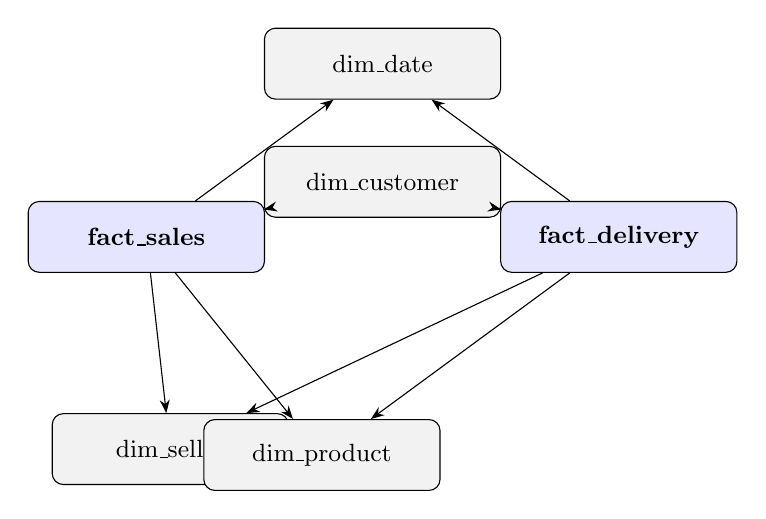
\begin{tikzpicture}[
  box/.style={draw, rounded corners, minimum width=3cm, minimum height=0.9cm, font=\small},
  fact/.style={box, fill=blue!10, font=\small\bfseries},
  dim/.style={box, fill=gray!10},
  >=Stealth]
\node[fact] (fs) at (-3,0) {fact\_sales};
\node[fact] (fd) at (3,0) {fact\_delivery};
\node[dim] (dd) at (0,2.2) {dim\_date};
\node[dim] (dc) at (0,0.7) {dim\_customer};
\node[dim] (ds) at (0,-0,7) {dim\_seller};
\node[dim] (dp) at (0,-2,2) {dim\_product};
\foreach \d in {dd,dc,ds,dp}{\draw[->] (fs) -- (\d); \draw[->] (fd) -- (\d);}
\end{tikzpicture}
\caption{Schema fact constellation: 2 fact dùng chung 4 dimension. \code{fact\_delivery} dùng \code{dim\_date} 2 lần (ngày mua, ngày giao).}
\end{figure}

\hinh{Schema chi tiết (vẽ bằng dbdiagram.io hoặc chụp từ DBeaver)}

\subsection*{Grain (granularity)}

\begin{table}[H]
\centering
\begin{tabular}{L{3cm}L{4.5cm}L{7cm}}
\toprule
Fact & Grain (1 dòng =) & Lý do \\
\midrule
\code{fact\_sales} & 1 sản phẩm trong 1 đơn hàng & Mức chi tiết nhất của doanh thu; phân tích được theo sản phẩm và người bán \\
\code{fact\_delivery} & 1 đơn hàng \textbf{đã giao} & Ngày giao và review thuộc về \textbf{cả đơn}, không thuộc từng sản phẩm \\
\bottomrule
\end{tabular}
\end{table}

\textbf{Vì sao không gộp thành 1 fact?} Nếu đặt review vào \code{fact\_sales}, một đơn có 3 sản phẩm sẽ lặp review 3 lần. Khi đó điểm trung bình và tỷ lệ review xấu bị tính sai do đếm trùng. Đây chính là vấn đề granularity nêu trong slide Ch.2.

\section{Các bảng dimension}

Mọi dimension dùng \textbf{surrogate key} kiểu số nguyên tự tăng (Kimball).

\begin{table}[H]
\centering\small
\begin{tabular}{L{2.4cm}L{2.2cm}L{4.9cm}L{2.8cm}r}
\toprule
Dimension & Khoá & Thuộc tính & Hierarchy & Số dòng \\
\midrule
\code{dim\_date} & date\_key (yyyymmdd) & full\_date, day, month, month\_name, quarter, year, year\_month, weekday, is\_weekend & year $>$ quarter $>$ month $>$ day & 1.096 \\
\code{dim\_customer} & customer\_key & customer\_unique\_id, zip\_code\_prefix, city, state, region & region $>$ state $>$ city & 96.096 \\
\code{dim\_seller} & seller\_key & seller\_id, zip\_code\_prefix, city, state, region & region $>$ state $>$ city & 3.095 \\
\code{dim\_product} & product\_key & product\_id, category\_pt, category\_en, photos\_qty, weight\_g, volume\_cm3 & category $>$ product & 32.951 \\
\bottomrule
\end{tabular}
\end{table}

\begin{table}[H]
\centering\small
\caption{Ánh xạ bang $\rightarrow$ vùng (5 vùng hành chính của Brazil)}
\begin{tabular}{ll}
\toprule
Vùng & Các bang \\
\midrule
North & AC, AP, AM, PA, RO, RR, TO \\
Northeast & AL, BA, CE, MA, PB, PE, PI, RN, SE \\
Central-West & DF, GO, MT, MS \\
Southeast & ES, MG, RJ, SP \\
South & PR, RS, SC \\
\bottomrule
\end{tabular}
\end{table}

\section{Các bảng fact}

\begin{table}[H]
\centering\small
\caption{\code{fact\_sales} (112.650 dòng)}
\begin{tabular}{L{6cm}L{3.5cm}L{5cm}}
\toprule
Cột & Loại & Ý nghĩa \\
\midrule
purchase\_date\_key, customer\_key, seller\_key, product\_key & FK & Khoá tới 4 dimension \\
order\_id, order\_item\_id, order\_status & Degenerate dimension & Thông tin đơn hàng, không cần bảng riêng \\
price & Measure, additive & Giá sản phẩm \\
freight\_value & Measure, additive & Phí vận chuyển \\
total\_value & Measure, additive & price + freight\_value \\
\bottomrule
\end{tabular}
\end{table}

\begin{table}[H]
\centering\small
\caption{\code{fact\_delivery} (96.470 dòng)}
\begin{tabular}{L{5cm}L{3.5cm}L{6cm}}
\toprule
Cột & Loại & Ý nghĩa \\
\midrule
order\_id & Degenerate, PK & Mã đơn \\
purchase\_date\_key, delivered\_date\_key & FK $\rightarrow$ dim\_date & Dùng chiều ngày 2 lần (ngày mua, ngày giao) \\
customer\_key & FK & Khách hàng \\
seller\_key, product\_key & FK & Người bán và sản phẩm của \textbf{item chính} (item giá cao nhất trong đơn) \\
n\_items, n\_sellers & Measure, additive & Số sản phẩm, số người bán trong đơn \\
order\_value, freight\_total & Measure, additive & Tổng giá, tổng phí ship \\
delivery\_days & Measure & Số ngày từ lúc mua đến lúc giao \\
estimated\_days & Measure & Số ngày từ lúc mua đến ngày giao dự kiến \\
delay\_days & Measure & Ngày giao $-$ ngày dự kiến ($>0$ là trễ) \\
is\_late & Measure 0/1 & 1 nếu giao trễ \\
review\_score & Measure & Điểm 1--5 (NULL nếu đơn không có review) \\
is\_bad\_review & Measure 0/1 & 1 nếu điểm $\le 2$ \\
\bottomrule
\end{tabular}
\end{table}

\textbf{Phân loại measure:} tổng tiền, số sản phẩm, số đơn đã giao là \textbf{additive} (cộng dồn được). Trung bình, tỷ lệ và số đơn \emph{distinct} là \textbf{non-additive}: không lấy tổng của các nhóm con được, phải tính lại từ fact. Trang OLAP thể hiện rõ sự khác biệt này (Mục~\ref{sec:olap-page}).

\section{Quy trình ETL}\label{sec:etl}

Theo slide Ch.2: \emph{Extract} lấy dữ liệu mà không làm gián đoạn hệ thống nguồn; \emph{Transform} gồm data cleansing, data mapping và business rules application; \emph{Load} có thể nạp incremental hoặc full refresh. Dữ liệu đi qua \textbf{data staging area} (slide Ch.1).

Toàn bộ ETL chạy bằng \textbf{1 lệnh} \code{python src/etl/run\_etl.py}, mất khoảng 12 giây (gồm cả bước kiểm tra hợp đồng nguồn và kiểm tra chất lượng).

\hinh{Luồng ETL: CSV $\rightarrow$ staging $\rightarrow$ dw $\rightarrow$ meta}

\begin{table}[H]
\centering\small
\caption{Các bước ETL}
\begin{tabular}{L{2.8cm}L{3.6cm}L{8.2cm}}
\toprule
Bước & File & Việc làm \\
\midrule
0. Kiểm tra nguồn & \code{contracts.py} & Đọc từng CSV bằng CSV parser trước khi nạp. Thiếu file hoặc header sai thì \textbf{dừng hẳn}, chưa động vào CSDL. Vi phạm về giá trị được ghi thành check (Mục~\ref{sec:quality}) \\
1. Extract & \code{01\_staging.sql}, \code{run\_etl.py} & Tạo schema \code{staging}, mỗi CSV một bảng, \textbf{mọi cột kiểu TEXT} (giữ nguyên nguồn); nạp hàng loạt bằng \code{COPY \ldots{} FORMAT csv} \\
2. Tạo schema DW & \code{02\_dw\_schema.sql} & Xoá và tạo lại schema \code{dw}: 4 dimension, 2 fact, index, partition; tạo \code{meta.etl\_log} nếu chưa có \\
3. Transform + Load & \code{03\_transform\_load.sql} & Làm sạch, ánh xạ, áp quy tắc nghiệp vụ, nạp vào dimension rồi fact \\
4. Tổng hợp sẵn & \code{04\_olap\_views.sql} & Tạo 3 materialized view \\
5. Metadata & \code{run\_etl.py} & Ghi số dòng nguồn $\rightarrow$ đích của từng bảng vào \code{meta.etl\_log} \\
6. Kiểm tra chất lượng & \code{05\_checks.sql} & Ghi 27 kiểm tra trên DW vào \code{meta.check\_result}. Cả 6 bước chạy trong \textbf{1 transaction}: lỗi thì rollback toàn bộ. Có check không đạt thì lệnh trả mã lỗi 1 \\
\bottomrule
\end{tabular}
\end{table}

\begin{table}[H]
\centering\small
\caption{Các quy tắc Transform (đều nằm trong \code{03\_transform\_load.sql})}
\begin{tabular}{L{3.2cm}L{11.4cm}}
\toprule
Nhóm (slide Ch.2) & Quy tắc \\
\midrule
Data cleansing & Đơn có nhiều review $\rightarrow$ giữ review có \code{review\_answer\_timestamp} mới nhất; danh mục rỗng $\rightarrow$ \code{unknown}; bổ sung bản dịch cho 2 danh mục thiếu; ép kiểu TEXT $\rightarrow$ DATE / NUMERIC / INTEGER, chuỗi rỗng $\rightarrow$ NULL \\
Data mapping & Danh mục PT $\rightarrow$ EN; timestamp $\rightarrow$ \code{date\_key} (yyyymmdd); bang $\rightarrow$ vùng; zip giữ dạng TEXT \\
Business rules & Khách hàng thật = \code{customer\_unique\_id}, giữ địa chỉ của đơn gần nhất; \code{fact\_delivery} chỉ gồm đơn \code{delivered} có ngày giao; \code{is\_late = 1} khi ngày giao $>$ ngày dự kiến; review xấu = điểm $\le 2$; item chính = item giá cao nhất (hoà thì lấy \code{order\_item\_id} nhỏ nhất); \code{fact\_sales} giữ mọi trạng thái đơn, các phân tích doanh thu loại \code{canceled} / \code{unavailable} \\
Attribute construction (slide Ch.2) & \code{delivery\_days}, \code{estimated\_days}, \code{delay\_days}, \code{is\_late}, \code{is\_bad\_review}, \code{n\_items}, \code{n\_sellers}, \code{volume\_cm3} = dài $\times$ rộng $\times$ cao, \code{region} \\
Discretization (tầng phân tích) & Nhóm mức trễ: sớm $>$ 7 ngày / sớm 1--7 / đúng ngày / trễ 1--3 / 4--7 / 8--14 / $>$ 14 ngày \\
\bottomrule
\end{tabular}
\end{table}

\textbf{Load:} dùng \emph{full refresh}: mỗi lần chạy, \code{staging} và \code{dw} được xoá và nạp lại. Cách này đơn giản và chạy lại bao nhiêu lần cũng cho cùng kết quả. \emph{Incremental load} là hướng phát triển.

\section{Thiết kế vật lý và metadata}

\begin{table}[H]
\centering\small
\begin{tabular}{L{3.6cm}L{6.6cm}L{4.4cm}}
\toprule
Kỹ thuật & Hiện thực & Mục đích \\
\midrule
Surrogate key & \code{SERIAL} cho dim\_customer / seller / product; \code{date\_key} dạng yyyymmdd & Khoá gọn, độc lập với khoá nguồn \\
Partitioning theo thời gian (slide Ch.1) & \code{fact\_sales} có \code{PARTITION BY RANGE (purchase\_date\_key)}, 3 partition 2016 / 2017 / 2018 & Truy vấn theo năm chỉ quét partition cần thiết \\
Index & Index trên các FK của 2 fact & Tăng tốc join / slice / dice \\
Materialized views & \code{mv\_monthly\_kpi}, \code{mv\_sales\_cube}, \code{mv\_delivery\_by\_state} & Tổng hợp sẵn (ROLAP, Mục~\ref{sec:rolap}) \\
Metadata (slide Ch.2: ``history of extracts'') & \code{meta.etl\_log(run\_id, step, table\_name, source\_rows, loaded\_rows, note)} đặt ở schema riêng nên \textbf{không bị xoá} khi full refresh & Truy vết từng lần nạp \\
Metadata chất lượng & \code{meta.check\_result(run\_id, category, check\_name, expected, actual, passed)} & Lưu kết quả kiểm tra của từng lần nạp \\
Lineage dữ liệu $\rightarrow$ mô hình & \code{models/metrics.json} lưu \code{etl\_run\_id} của lần ETL dùng để train & Trang Data Quality cảnh báo khi mô hình được train từ dữ liệu cũ \\
\bottomrule
\end{tabular}
\end{table}

\begin{table}[H]
\centering\small
\begin{minipage}[t]{0.38\linewidth}\centering
\caption{Số dòng mỗi partition}
\begin{tabular}{lr}
\toprule
Partition & Số dòng \\
\midrule
fact\_sales\_2016 & 370 \\
fact\_sales\_2017 & 50.864 \\
fact\_sales\_2018 & 61.416 \\
\midrule
\textbf{Tổng} & \textbf{112.650} \\
\bottomrule
\end{tabular}
\end{minipage}\hfill
\begin{minipage}[t]{0.58\linewidth}\centering
\caption{Dung lượng trên đĩa (gồm index)}
\begin{tabular}{L{4.6cm}r}
\toprule
Bảng & Dung lượng \\
\midrule
fact\_delivery & 24 MB \\
dim\_customer & 17 MB \\
fact\_sales\_2018 / 2017 / 2016 & 14 MB / 11 MB / 168 kB \\
dim\_product & 6,8 MB \\
dim\_seller & 680 kB \\
dim\_date & 144 kB \\
mv\_sales\_cube / mv\_monthly\_kpi / mv\_delivery\_by\_state & 136 / 16 / 16 kB \\
\bottomrule
\end{tabular}
\end{minipage}
\end{table}

% =====================================================================
\chapter{Xây dựng Backend và Frontend}\label{ch:system}
% =====================================================================

\section{Kiến trúc ba tầng}\label{sec:arch}

Hệ thống theo \textbf{kiến trúc ba tầng} (slide Ch.2--3). Phía trên data mart là dashboard OLAP và DSS.

\begin{figure}[H]
\centering
\begin{tikzpicture}[
  tier/.style={draw, rounded corners, align=left, font=\small, inner sep=6pt, text width=4.1cm},
  >=Stealth]
\node[tier, fill=gray!10] (b) {\textbf{Bottom tier}\\8 file CSV Olist\\Kiểm tra hợp đồng nguồn\\Extract: \code{COPY}};
\node[tier, fill=blue!8, right=0.6cm of b] (m) {\textbf{Middle tier} (PostgreSQL)\\schema \code{staging}\\$\downarrow$ Transform + Load\\schema \code{dw} (fact constellation)\\+ materialized views (ROLAP)\\schema \code{meta} (etl\_log, check\_result)};
\node[tier, fill=green!8, right=0.6cm of m] (t) {\textbf{Top tier} (Streamlit)\\Home (KPI)\\OLAP (5 phép toán)\\Delivery\\DSS (5 tab)\\Data Quality};
\draw[->, thick] (b) -- (m);
\draw[->, thick] (m) -- (t);
\end{tikzpicture}
\caption{Kiến trúc ba tầng của hệ thống}
\end{figure}

\hinh{Vẽ lại sơ đồ kiến trúc (nếu cần đẹp hơn)}

\section{Công nghệ}

\begin{table}[H]
\centering\small
\begin{tabular}{L{3cm}L{5.2cm}L{6.4cm}}
\toprule
Thành phần & Công nghệ & Ghi chú \\
\midrule
CSDL / DW & PostgreSQL 16 & Partitioning, materialized view, \code{GROUP BY CUBE} \\
ETL & Python 3.12 (psycopg2, SQLAlchemy) + SQL & Python điều phối, SQL biến đổi \\
Mô hình DSS & scikit-learn 1.5, pandas & \code{DecisionTreeClassifier} (entropy) \\
Tối ưu & SciPy (\code{milp}, solver HiGHS) & Giải chính xác bài toán phân bổ ngân sách \\
Giao diện & Streamlit 1.39, Plotly & Web app nhiều trang \\
Kiểm thử & pytest & 102 test: unit và kiểm tra trên CSDL thật \\
Môi trường & micromamba (cục bộ trong project) & Cài Python + PostgreSQL bằng 1 lệnh, không đụng hệ thống \\
Tuỳ chọn & Docker Compose, Metabase & Chạy toàn bộ stack bằng container, kèm 3 dashboard Metabase; không dùng cho số liệu trong báo cáo này \\
\bottomrule
\end{tabular}
\end{table}

\section{Backend: kết quả ETL}

\begin{table}[H]
\centering\small
\caption{Nội dung \code{meta.etl\_log} của lần chạy gần nhất}
\begin{tabular}{llrrL{5cm}}
\toprule
Bước & Bảng & Dòng nguồn & Dòng nạp & Ghi chú \\
\midrule
extract & staging.orders & 99.441 & 99.441 & \\
extract & staging.order\_items & 112.650 & 112.650 & \\
extract & staging.order\_payments & 103.886 & 103.886 & \\
extract & staging.order\_reviews & 99.224 & 99.224 & \\
extract & staging.customers & 99.441 & 99.441 & \\
extract & staging.sellers & 3.095 & 3.095 & \\
extract & staging.products & 32.951 & 32.951 & \\
extract & staging.category\_translation & 71 & 71 & \\
load & dw.dim\_date & -- & 1.096 & Sinh lịch 2016--2018 \\
load & dw.dim\_customer & 99.441 & 96.096 & Gộp về customer\_unique\_id \\
load & dw.dim\_seller & 3.095 & 3.095 & \\
load & dw.dim\_product & 32.951 & 32.951 & \\
load & dw.fact\_sales & 112.650 & 112.650 & \\
load & dw.fact\_delivery & 99.441 & 96.470 & Chỉ đơn delivered có ngày giao \\
\bottomrule
\end{tabular}
\end{table}

\begin{table}[H]
\centering\small
\caption{Kiểm tra tính đúng đắn của ETL}
\begin{tabular}{L{7cm}L{7.6cm}}
\toprule
Kiểm tra & Kết quả \\
\midrule
Số dòng staging = số dòng CSV (đếm bằng CSV parser) & Khớp cả 8 file \\
\code{SUM(price)} staging = \code{SUM(price)} \code{dw.fact\_sales} & 13.591.643,70 = 13.591.643,70 \\
\code{fact\_delivery} = số đơn delivered $-$ số đơn delivered thiếu ngày giao & 96.478 $-$ 8 = 96.470 \\
Chạy lại ETL lần 2 & Cùng số dòng; \code{etl\_log} có thêm 1 lượt chạy \\
Thời gian chạy & $\sim$5 giây cho riêng phần nạp (4,6--4,9 s, đo ngày 02/11); $\sim$12 giây khi gồm cả kiểm tra hợp đồng nguồn và kiểm tra chất lượng (12,3 s, đo ngày 14/11) \\
\bottomrule
\end{tabular}
\end{table}

\section{Backend: kiểm soát chất lượng dữ liệu}\label{sec:quality}

Mỗi lần chạy ETL đều tự kiểm tra lại dữ liệu và lưu kết quả vào \code{meta.check\_result}. Nhờ vậy, người dùng dashboard và mô hình DSS biết dữ liệu có đáng tin hay không mà không cần kiểm tra tay.

\textbf{Nguyên tắc.} Giá trị kỳ vọng của mỗi kiểm tra được \textbf{tính lại độc lập từ staging}, không dùng lại logic transform. Nếu tính kỳ vọng bằng chính logic transform thì một lỗi trong transform sẽ tự ``khớp'' với chính nó và không bị phát hiện.

\begin{table}[H]
\centering\small
\caption{Hai lớp kiểm tra}
\begin{tabular}{L{2.8cm}L{3.7cm}L{1.8cm}L{5.9cm}}
\toprule
Lớp & File & Khi nào chạy & Nội dung \\
\midrule
Hợp đồng nguồn (\emph{source contract}) & \code{src/etl/}\allowbreak\code{contracts.py} & Trước khi nạp & Mỗi CSV phải có đúng header như mô tả; khoá có mặt và không trùng; số và thời gian đọc được; điểm review 1--5; bang là mã UF 2 chữ; zip đủ 5 chữ số \\
Kiểm tra trên DW & \code{src/sql/05\_checks.sql} & Sau khi nạp & Grain, đối chiếu staging $\leftrightarrow$ DW, miền giá trị, độ phủ, tổng của materialized view \\
\bottomrule
\end{tabular}
\end{table}

\begin{table}[H]
\centering\small
\caption{Kết quả kiểm tra lần chạy 14/11/2026: 43/43 đạt (danh sách đầy đủ ở Phụ lục~\ref{app:checks})}
\begin{tabular}{lrL{10.5cm}}
\toprule
Nhóm & Số KT & Ví dụ \\
\midrule
source & 16 & Mỗi file trong 8 CSV: không vi phạm hợp đồng; số dòng CSV = số dòng staging \\
grain & 3 & Không trùng (order\_id, order\_item\_id) trong fact\_sales; không trùng order\_id trong fact\_delivery; không trùng customer\_unique\_id \\
reconciliation & 10 & Số dòng, SUM(price), SUM(freight\_value) giữa staging và fact\_sales; số đơn trễ; số đơn có review \\
domain & 7 & review\_score trong 1..5; is\_bad\_review nhất quán với điểm $\le 2$; delay\_days = delivery\_days $-$ estimated\_days; total\_value = price + freight\_value \\
coverage & 3 & Mọi ngày mua / giao nằm trong dim\_date; mọi danh mục có tên tiếng Anh; mọi bang có vùng \\
aggregate & 4 & Tổng của mv\_sales\_cube, mv\_monthly\_kpi, mv\_delivery\_by\_state khớp với fact; các tỷ lệ nằm trong [0, 1] \\
\midrule
\textbf{Tổng} & \textbf{43} & \\
\bottomrule
\end{tabular}
\end{table}

\textbf{Kiểm thử tự động.} Thư mục \code{tests/} có 102 test (pytest), gồm unit test và test chạy trên CSDL thật. Với mỗi quy tắc nghiệp vụ, \code{tests/test\_etl\_checks.py} cố tình làm hỏng dữ liệu để xác nhận kiểm tra tương ứng báo lỗi. Lần chạy 14/11: \textbf{100 test đạt, 2 test bỏ qua}. Một test cần ETL chạy 2 lần; test còn lại chỉ chạy trong môi trường Docker.

\section{Backend: OLAP theo kiến trúc ROLAP}\label{sec:rolap}

Theo slide Ch.3, các phép toán OLAP gồm \textbf{roll-up}, \textbf{drill-down}, \textbf{slice}, \textbf{dice} và \textbf{pivot}; OLAP server có 3 loại: \textbf{ROLAP} (lưu trên CSDL quan hệ), \textbf{MOLAP} (mảng đa chiều) và \textbf{HOLAP} (kết hợp).

Hệ thống dùng \textbf{ROLAP}: dữ liệu chi tiết nằm trong bảng quan hệ của PostgreSQL, mỗi thao tác OLAP được dịch thành 1 câu \code{SELECT \ldots{} GROUP BY} nối fact với các dimension. Các phép tổng hợp hay dùng được \textbf{tính sẵn} bằng materialized view:

\begin{table}[H]
\centering\small
\begin{tabular}{L{3.6cm}L{8.6cm}L{2.2cm}}
\toprule
Materialized view & Nội dung & Dùng ở \\
\midrule
\code{mv\_monthly\_kpi} & Theo tháng: doanh thu, phí ship, số sản phẩm, số đơn, số đơn giao, tỷ lệ trễ, số ngày giao TB, review TB, tỷ lệ review xấu (kết hợp 2 fact) & Home \\
\code{mv\_sales\_cube} & \code{GROUP BY CUBE (year, customer\_region, category)}: mọi tổ hợp cùng các dòng tổng phụ (NULL = ``Tất cả'') & OLAP \\
\code{mv\_delivery\_by\_state} & Theo bang: số đơn, tỷ lệ trễ, ngày giao TB, review TB, tỷ lệ review xấu, doanh thu & Delivery \\
\bottomrule
\end{tabular}
\end{table}

\section{Frontend: dashboard Streamlit}

Dashboard gồm 5 trang:

\begin{table}[H]
\centering\small
\begin{tabular}{L{2.6cm}L{9cm}L{3cm}}
\toprule
Trang & Nội dung & Trả lời câu hỏi \\
\midrule
Home & KPI tổng và xu hướng theo tháng & Phân tích 1 \\
OLAP & Roll-up, drill-down, slice, dice, pivot trên 2 fact & Phân tích 1, 2 \\
Delivery & Giao hàng và review theo mức trễ, bang, danh mục & Phân tích 2, 3 \\
DSS & 5 tab: mô hình, xếp hạng, what-if \& sensitivity, goal seeking, tối ưu ngân sách & Quyết định 1--5 \\
Data Quality & Kết quả kiểm tra, số dòng qua từng bước, lịch sử chạy, quy tắc làm sạch, mô hình train từ lần ETL nào & Độ tin cậy dữ liệu \\
\bottomrule
\end{tabular}
\end{table}

\subsection{Trang OLAP}\label{sec:olap-page}

\begin{table}[H]
\centering\small
\caption{Định nghĩa khối dữ liệu trong ứng dụng}
\begin{tabular}{L{4cm}L{10.6cm}}
\toprule
Thành phần & Lựa chọn \\
\midrule
Fact & \code{fact\_sales} hoặc \code{fact\_delivery} (2 fact dùng chung dimension, minh hoạ fact constellation) \\
Measures -- fact\_sales & Doanh thu (SUM price); Phí vận chuyển (SUM); Số sản phẩm (COUNT); Số đơn (COUNT DISTINCT); Giá TB / sản phẩm (AVG) \\
Measures -- fact\_delivery & Số đơn đã giao (COUNT); Tỷ lệ giao trễ (\%); Số ngày giao TB; Điểm review TB; Tỷ lệ review xấu (\%) \\
Hierarchy Thời gian & Năm $\rightarrow$ Quý $\rightarrow$ Tháng \\
Hierarchy Địa lý khách hàng / người bán & Vùng $\rightarrow$ Bang $\rightarrow$ Thành phố \\
Hierarchy Sản phẩm & Danh mục \\
\bottomrule
\end{tabular}
\end{table}

\begin{table}[H]
\centering\small
\caption{Hiện thực 5 phép toán OLAP}
\begin{tabular}{L{2.2cm}L{5.4cm}L{7cm}}
\toprule
Phép toán & Thao tác trên giao diện & SQL tương ứng \\
\midrule
Roll-up & Nút ``Roll-up'' (vd. Tháng $\rightarrow$ Quý $\rightarrow$ Năm) & \code{GROUP BY} theo cột cấp cao hơn \\
Drill-down & Nút ``Drill-down'' (vd. Năm $\rightarrow$ Quý $\rightarrow$ Tháng) & \code{GROUP BY} theo cột cấp thấp hơn \\
Slice & Chọn ``Cố định năm'' = 2017 & \code{WHERE d.year = :year} \\
Dice & Chọn nhiều bang và nhiều danh mục & \code{WHERE c.state = ANY(:states) AND p.category\_en = ANY(:categories)} \\
Pivot & Nút ``Pivot'' đổi chiều hàng $\leftrightarrow$ cột & Đổi vai trò 2 cột trong \code{GROUP BY 1, 2} + \code{pivot\_table} \\
\bottomrule
\end{tabular}
\end{table}

Một số chi tiết khác của trang:
\begin{itemize}
\item \textbf{Hiển thị:} bảng pivot kèm heatmap (khi có chiều cột), hoặc biểu đồ cột (khi chỉ có chiều hàng).
\item \textbf{SQL sinh ra:} hiện trong mục ``SQL được sinh ra''.
\item \textbf{Additive vs non-additive:} chỉ measure additive mới có dòng / cột ``Tổng''. Với measure non-additive, trang hiện ghi chú vì sao không cộng dồn được.
\item \textbf{An toàn SQL:} chỉ các biểu thức có sẵn trong cấu hình (whitelist) mới được đưa vào SQL; giá trị người dùng chọn được truyền qua tham số.
\end{itemize}

\hinh{Mỗi phép toán một ảnh: roll-up, drill-down, slice, dice, pivot. Thêm 1 ảnh mục ``SQL được sinh ra'' và 1 ảnh khi chọn fact\_delivery}

\subsubsection*{Ví dụ kết quả các phép toán}

Doanh thu ở đây là tổng giá sản phẩm, loại đơn canceled / unavailable.

\begin{table}[H]
\centering\small
\caption{Roll-up về cấp cao nhất (dòng ``Tất cả'' do \code{CUBE} sinh ra)}
\begin{tabular}{lrrrr}
\toprule
Năm & Doanh thu (R\$) & Số sản phẩm & Số đơn & Giá trị TB / đơn (R\$) \\
\midrule
2016 & 44.726,06 & 348 & 293 & 152,65 \\
2017 & 6.108.492,27 & 50.617 & 44.375 & 137,66 \\
2018 & 7.341.182,41 & 61.136 & 53.531 & 137,14 \\
\midrule
\textbf{Tất cả} & \textbf{13.494.400,74} & \textbf{112.101} & \textbf{98.199} & \textbf{137,42} \\
\bottomrule
\end{tabular}
\end{table}
\bieudo{cột}

\begin{table}[H]
\centering\small
\begin{minipage}[t]{0.5\linewidth}\centering
\caption{Drill-down Năm $\rightarrow$ Quý}
\begin{tabular}{lrr}
\toprule
Quý & Doanh thu (R\$) & Số đơn \\
\midrule
2016-Q3 & 207,86 & 2 \\
2016-Q4 & 44.518,20 & 291 \\
2017-Q1 & 733.398,94 & 5.122 \\
2017-Q2 & 1.286.918,78 & 9.222 \\
2017-Q3 & 1.681.949,00 & 12.445 \\
2017-Q4 & 2.406.225,55 & 17.586 \\
2018-Q1 & 2.764.402,78 & 20.979 \\
2018-Q2 & 2.849.730,26 & 19.897 \\
2018-Q3 & 1.727.049,37 & 12.655 \\
\bottomrule
\end{tabular}
\end{minipage}\hfill
\begin{minipage}[t]{0.46\linewidth}\centering
\caption{Drill-down 2018-Q1 $\rightarrow$ Tháng}
\begin{tabular}{lr}
\toprule
Tháng & Doanh thu (R\$) \\
\midrule
2018-01 & 945.456,29 \\
2018-02 & 837.895,43 \\
2018-03 & 981.051,06 \\
\bottomrule
\end{tabular}

\vspace{0.6em}
\caption{Slice năm 2017, theo vùng khách hàng}
\begin{tabular}{lr}
\toprule
Vùng & Doanh thu 2017 (R\$) \\
\midrule
Southeast & 3.930.293,30 \\
South & 881.752,70 \\
Northeast & 727.528,43 \\
Central-West & 400.781,10 \\
North & 168.136,74 \\
\bottomrule
\end{tabular}
\end{minipage}
\end{table}

Ghi chú: dữ liệu 2018-Q3 chỉ đến hết tháng 8, và tháng 9/2018 chỉ có 1 đơn.

\begin{table}[H]
\centering\small
\caption{Pivot vùng $\times$ năm (doanh thu, R\$). Đổi trục sẽ cho bảng năm $\times$ vùng}
\begin{tabular}{lrrrr}
\toprule
Vùng \textbackslash{} Năm & 2016 & 2017 & 2018 & Tổng \\
\midrule
Southeast & 27.700,71 & 3.930.293,30 & 4.866.163,13 & 8.824.157,14 \\
South & 7.455,89 & 881.752,70 & 1.047.635,66 & 1.936.844,25 \\
Northeast & 6.013,32 & 727.528,43 & 804.697,84 & 1.538.239,59 \\
Central-West & 2.355,95 & 400.781,10 & 458.089,53 & 861.226,58 \\
North & 1.200,19 & 168.136,74 & 164.596,25 & 333.933,18 \\
\midrule
\textbf{Tổng} & 44.726,06 & 6.108.492,27 & 7.341.182,41 & 13.494.400,74 \\
\bottomrule
\end{tabular}
\end{table}
\bieudo{heatmap / cột chồng}

\begin{table}[H]
\centering\small
\caption{Dice: bang $\in$ \{SP, RJ\}, danh mục $\in$ \{health\_beauty, bed\_bath\_table\} (doanh thu, R\$)}
\begin{tabular}{llrr}
\toprule
Năm & Bang & bed\_bath\_table & health\_beauty \\
\midrule
2016 & RJ & 59,90 & 1.237,79 \\
2016 & SP & 29,90 & 1.079,04 \\
2017 & RJ & 80.141,28 & 64.378,98 \\
2017 & SP & 207.777,67 & 157.016,53 \\
2018 & RJ & 67.562,26 & 79.176,36 \\
2018 & SP & 270.371,52 & 302.498,32 \\
\bottomrule
\end{tabular}
\end{table}

\begin{table}[H]
\centering\small
\begin{minipage}[t]{0.4\linewidth}\centering
\caption{Top 10 bang theo doanh thu}
\begin{tabular}{lrr}
\toprule
Bang & Doanh thu (R\$) & Số đơn \\
\midrule
SP & 5.165.781,70 & 41.130 \\
RJ & 1.811.484,23 & 12.698 \\
MG & 1.573.269,18 & 11.493 \\
RS & 742.639,78 & 5.415 \\
PR & 675.928,19 & 4.980 \\
SC & 518.276,28 & 3.600 \\
BA & 506.878,84 & 3.342 \\
DF & 300.085,75 & 2.117 \\
GO & 288.157,45 & 1.997 \\
ES & 273.622,03 & 2.019 \\
\bottomrule
\end{tabular}
\end{minipage}\hfill
\begin{minipage}[t]{0.58\linewidth}\centering
\caption{Top 10 danh mục theo doanh thu}
\setlength{\tabcolsep}{3pt}
\begin{tabular}{lrrr}
\toprule
Danh mục & Doanh thu (R\$) & Số SP & Số đơn \\
\midrule
health\_beauty & 1.255.695,13 & 9.634 & 8.800 \\
watches\_gifts & 1.198.185,21 & 5.970 & 5.604 \\
bed\_bath\_table & 1.035.964,06 & 11.097 & 9.399 \\
sports\_leisure & 979.740,92 & 8.590 & 7.673 \\
computers\_accessories & 904.322,02 & 7.781 & 6.654 \\
furniture\_decor & 727.465,05 & 8.298 & 6.425 \\
housewares & 626.825,80 & 6.915 & 5.847 \\
cool\_stuff & 620.770,49 & 3.779 & 3.616 \\
auto & 586.585,73 & 4.204 & 3.872 \\
garden\_tools & 481.009,94 & 4.328 & 3.505 \\
\bottomrule
\end{tabular}
\end{minipage}
\end{table}

\subsection{Trang Home}

\begin{table}[H]
\centering\small
\caption{KPI tổng}
\begin{tabular}{L{9cm}r}
\toprule
KPI & Giá trị \\
\midrule
Doanh thu (giá sản phẩm, loại canceled / unavailable) & R\$ 13.494.400,74 \\
Phí vận chuyển & R\$ 2.241.126,29 \\
Số đơn hàng & 98.199 \\
Số sản phẩm bán & 112.101 \\
Giá trị TB / đơn & R\$ 137,42 \\
Khách hàng có mua / người bán có bán / sản phẩm đã bán & 95.420 / 3.095 / 32.951 \\
Số đơn đã giao & 96.470 \\
Tỷ lệ giao trễ & 6,77\% \\
Số ngày giao TB / số ngày dự kiến TB & 12,50 / 24,37 ngày \\
Điểm review TB & 4,156 \\
Tỷ lệ review xấu ($\le 2$ sao) & 12,81\% \\
Đơn đã giao không có review & 646 \\
\bottomrule
\end{tabular}
\end{table}

\hinh{Trang Home}

\textbf{Xu hướng theo tháng.} Dashboard chỉ vẽ giai đoạn 2017-01 $\rightarrow$ 2018-08, vì các tháng ở hai đầu có rất ít đơn (2016-09: 2 đơn, 2016-12: 1 đơn, 2018-09: 1 đơn; tháng 2016-11 không có đơn).

\begingroup\small
\setlength{\tabcolsep}{4pt}
\begin{longtable}{lrrrrrrr}
\caption{Xu hướng theo tháng}\\
\toprule
Tháng & Doanh thu (R\$) & Số đơn & Đơn đã giao & Tỷ lệ trễ & Ngày giao TB & Review TB & Review xấu \\
\midrule\endfirsthead
\toprule
Tháng & Doanh thu (R\$) & Số đơn & Đơn đã giao & Tỷ lệ trễ & Ngày giao TB & Review TB & Review xấu \\
\midrule\endhead
2016-10 & 44.507,30 & 290 & 265 & 0,75\% & 19,63 & 4,011 & 16,41\% \\
2017-01 & 120.098,27 & 787 & 750 & 2,93\% & 12,75 & 4,198 & 12,01\% \\
2017-02 & 244.959,35 & 1.718 & 1.653 & 2,96\% & 13,30 & 4,203 & 11,08\% \\
2017-03 & 368.341,32 & 2.617 & 2.546 & 4,56\% & 13,04 & 4,187 & 11,24\% \\
2017-04 & 353.842,98 & 2.377 & 2.303 & 6,56\% & 15,02 & 4,135 & 12,93\% \\
2017-05 & 503.159,19 & 3.640 & 3.545 & 2,99\% & 11,43 & 4,236 & 10,07\% \\
2017-06 & 429.916,61 & 3.205 & 3.135 & 3,03\% & 12,01 & 4,223 & 10,74\% \\
2017-07 & 492.287,30 & 3.946 & 3.872 & 2,79\% & 11,49 & 4,260 & 9,94\% \\
2017-08 & 568.245,79 & 4.272 & 4.193 & 2,91\% & 11,02 & 4,313 & 9,39\% \\
2017-09 & 621.415,91 & 4.227 & 4.150 & 4,39\% & 11,72 & 4,268 & 10,27\% \\
2017-10 & 660.179,62 & 4.547 & 4.478 & 4,18\% & 11,73 & 4,205 & 11,07\% \\
2017-11 & 1.003.862,14 & 7.421 & 7.288 & 12,40\% & 15,07 & 3,989 & 16,57\% \\
2017-12 & 742.183,79 & 5.618 & 5.513 & 7,46\% & 15,31 & 4,088 & 14,43\% \\
2018-01 & 945.456,29 & 7.187 & 7.069 & 5,70\% & 14,01 & 4,109 & 13,70\% \\
2018-02 & 837.895,43 & 6.624 & 6.555 & 14,13\% & 16,87 & 3,881 & 19,38\% \\
2018-03 & 981.051,06 & 7.168 & 7.003 & 18,96\% & 16,24 & 3,813 & 21,17\% \\
2018-04 & 993.592,98 & 6.919 & 6.798 & 4,50\% & 11,42 & 4,206 & 11,79\% \\
2018-05 & 992.871,75 & 6.833 & 6.749 & 6,56\% & 11,34 & 4,236 & 10,76\% \\
2018-06 & 863.265,53 & 6.145 & 6.096 & 1,16\% & 9,16 & 4,307 & 9,98\% \\
2018-07 & 878.044,27 & 6.233 & 6.156 & 3,38\% & 8,89 & 4,317 & 9,68\% \\
2018-08 & 848.860,10 & 6.421 & 6.351 & 6,19\% & 7,66 & 4,310 & 9,54\% \\
\bottomrule
\end{longtable}
\endgroup
\bieudo{cột doanh thu + đường tỷ lệ trễ và tỷ lệ review xấu}

\textbf{Insight:}
\begin{itemize}
\item Tỷ lệ trễ và tỷ lệ review xấu \textbf{tăng giảm cùng nhau}. Hai đỉnh là 11/2017 (trễ 12,4\% $\rightarrow$ review xấu 16,6\%; tháng có Black Friday, số đơn tăng vọt lên 7.421) và 02--03/2018 (trễ 14,1--19,0\% $\rightarrow$ review xấu 19,4--21,2\%).
\item Các tháng trễ thấp (06/2018: 1,16\%) có tỷ lệ review xấu thấp nhất ($\sim$10\%).
\end{itemize}

\subsection{Trang Delivery}

\begin{table}[H]
\centering\small
\caption{Review theo mức độ trễ (discretization)}
\begin{tabular}{lrrr}
\toprule
Giao so với ngày dự kiến & Số đơn & Review TB & Tỷ lệ review xấu \\
\midrule
Sớm $>$ 7 ngày & 71.303 & 4,317 & 8,97\% \\
Sớm 1--7 ngày & 17.341 & 4,201 & 10,24\% \\
Đúng ngày & 1.292 & 4,034 & 12,42\% \\
Trễ 1--3 ngày & 1.870 & 3,291 & 32,13\% \\
Trễ 4--7 ngày & 1.802 & 2,103 & 67,68\% \\
Trễ 8--14 ngày & 1.478 & 1,671 & 80,15\% \\
Trễ $>$ 14 ngày & 1.384 & 1,724 & 78,35\% \\
\bottomrule
\end{tabular}
\end{table}
\bieudo{cột --- đây là biểu đồ ``đắt'' nhất để thuyết trình}

\begin{table}[H]
\centering\small
\caption{Phân bố điểm review: đúng hạn và trễ (đơn có review)}
\begin{tabular}{lrr}
\toprule
Điểm & Đúng hạn & Trễ \\
\midrule
1 sao & 5.920 & 3.431 \\
2 sao & 2.369 & 552 \\
3 sao & 7.222 & 694 \\
4 sao & 18.239 & 649 \\
5 sao & 55.693 & 1.055 \\
\midrule
Tổng & 89.443 & 6.381 \\
\bottomrule
\end{tabular}
\end{table}
\bieudo{cột chồng 100\%}

Với đơn trễ, \textbf{53,8\%} là 1 sao (3.431 / 6.381). Với đơn đúng hạn, \textbf{62,3\%} là 5 sao (55.693 / 89.443).

\begin{table}[H]
\centering\small
\caption{Giao hàng theo vùng khách hàng}
\begin{tabular}{lrrrrr}
\toprule
Vùng & Số đơn & Tỷ lệ trễ & Ngày giao TB & Review TB & Tỷ lệ review xấu \\
\midrule
Northeast & 9.045 & 12,71\% & 19,94 & 3,970 & 16,74\% \\
North & 1.797 & 8,57\% & 22,54 & 4,031 & 15,17\% \\
Central-West & 5.619 & 6,50\% & 14,95 & 4,129 & 13,12\% \\
Southeast & 66.197 & 6,12\% & 10,69 & 4,179 & 12,38\% \\
South & 13.812 & 5,90\% & 13,98 & 4,191 & 11,82\% \\
\bottomrule
\end{tabular}
\end{table}

\begingroup\small
\begin{longtable}{llrrrrr}
\caption{Giao hàng theo bang (sắp theo tỷ lệ trễ giảm dần)}\label{tab:states}\\
\toprule
Bang & Vùng & Số đơn & Tỷ lệ trễ & Ngày giao TB & Review TB & Review xấu \\
\midrule\endfirsthead
\toprule
Bang & Vùng & Số đơn & Tỷ lệ trễ & Ngày giao TB & Review TB & Review xấu \\
\midrule\endhead
AL & Northeast & 397 & 21,41\% & 24,50 & 3,848 & 21,32\% \\
MA & Northeast & 720 & 17,36\% & 21,48 & 3,835 & 19,86\% \\
SE & Northeast & 336 & 15,18\% & 21,42 & 3,907 & 18,86\% \\
PI & Northeast & 476 & 13,87\% & 19,39 & 3,994 & 16,14\% \\
CE & Northeast & 1.281 & 13,74\% & 21,18 & 3,946 & 17,10\% \\
RR & North & 41 & 12,20\% & 29,34 & 3,902 & 14,63\% \\
BA & Northeast & 3.254 & 12,17\% & 19,28 & 3,931 & 17,01\% \\
RJ & Southeast & 12.351 & 12,11\% & 15,24 & 3,965 & 18,33\% \\
PA & North & 946 & 11,21\% & 23,73 & 3,914 & 17,90\% \\
ES & Southeast & 1.996 & 10,72\% & 15,73 & 4,079 & 13,81\% \\
PB & Northeast & 515 & 10,29\% & 20,37 & 4,082 & 14,71\% \\
TO & North & 274 & 9,85\% & 17,60 & 4,154 & 12,09\% \\
MS & Central-West & 700 & 9,71\% & 15,54 & 4,160 & 13,32\% \\
PE & Northeast & 1.592 & 9,67\% & 18,38 & 4,080 & 14,89\% \\
RN & Northeast & 474 & 9,28\% & 19,22 & 4,151 & 12,95\% \\
SC & South & 3.547 & 8,20\% & 14,90 & 4,135 & 12,95\% \\
GO & Central-West & 1.956 & 6,49\% & 15,53 & 4,106 & 13,16\% \\
MT & Central-West & 886 & 6,09\% & 18,01 & 4,147 & 12,74\% \\
RS & South & 5.344 & 6,08\% & 15,25 & 4,185 & 11,92\% \\
DF & Central-West & 2.077 & 5,58\% & 12,89 & 4,134 & 13,16\% \\
MG & Southeast & 11.351 & 4,58\% & 11,95 & 4,192 & 11,76\% \\
SP & Southeast & 40.499 & 4,49\% & 8,70 & 4,246 & 10,69\% \\
PR & South & 4.921 & 4,04\% & 11,94 & 4,239 & 10,90\% \\
AC & North & 80 & 3,75\% & 21,00 & 4,088 & 15,00\% \\
AP & North & 67 & 2,99\% & 27,18 & 4,242 & 6,06\% \\
RO & North & 244 & 2,87\% & 19,28 & 4,165 & 11,93\% \\
AM & North & 145 & 2,76\% & 26,36 & 4,243 & 13,19\% \\
\bottomrule
\end{longtable}
\endgroup
\bieudo{cột tỷ lệ trễ theo bang, tô màu theo tỷ lệ review xấu}

\textbf{Insight:}
\begin{itemize}
\item Vùng Northeast trễ nhiều nhất (12,7\%).
\item \textbf{RJ} đáng chú ý: là bang lớn thứ 2 (12.351 đơn) nhưng trễ 12,1\% và có tỷ lệ review xấu cao nhất trong nhóm bang lớn (18,3\%).
\item SP giao nhanh nhất (8,7 ngày) và ít trễ (4,5\%).
\end{itemize}

\begingroup\small
\begin{longtable}{lrrrr}
\caption{Giao hàng theo danh mục ($\ge$ 500 đơn, sắp theo tỷ lệ review xấu)}\\
\toprule
Danh mục & Số đơn & Tỷ lệ trễ & Review TB & Review xấu \\
\midrule\endfirsthead
\toprule
Danh mục & Số đơn & Tỷ lệ trễ & Review TB & Review xấu \\
\midrule\endhead
office\_furniture & 1.251 & 8,07\% & 3,647 & 21,92\% \\
unknown & 1.358 & 7,14\% & 4,041 & 16,53\% \\
bed\_bath\_table & 9.184 & 7,48\% & 4,008 & 15,82\% \\
furniture\_decor & 6.188 & 7,24\% & 4,078 & 14,85\% \\
computers\_accessories & 6.511 & 6,40\% & 4,083 & 14,51\% \\
telephony & 4.073 & 7,14\% & 4,059 & 13,93\% \\
baby & 2.761 & 8,11\% & 4,122 & 13,76\% \\
watches\_gifts & 5.476 & 7,41\% & 4,123 & 13,65\% \\
electronics & 2.502 & 7,67\% & 4,129 & 13,05\% \\
auto & 3.792 & 7,33\% & 4,153 & 12,80\% \\
construction\_tools\_construction & 724 & 7,46\% & 4,152 & 12,66\% \\
garden\_tools & 3.400 & 6,62\% & 4,200 & 11,74\% \\
perfumery & 3.069 & 6,58\% & 4,268 & 11,57\% \\
housewares & 5.680 & 5,42\% & 4,204 & 11,57\% \\
musical\_instruments & 608 & 7,57\% & 4,243 & 11,46\% \\
health\_beauty & 8.613 & 7,54\% & 4,233 & 11,35\% \\
small\_appliances & 606 & 4,79\% & 4,266 & 11,31\% \\
toys & 3.787 & 6,42\% & 4,240 & 11,31\% \\
sports\_leisure & 7.492 & 6,59\% & 4,235 & 11,20\% \\
consoles\_games & 1.013 & 6,12\% & 4,182 & 11,06\% \\
home\_appliances & 747 & 4,42\% & 4,212 & 11,02\% \\
cool\_stuff & 3.530 & 5,92\% & 4,230 & 10,91\% \\
pet\_shop & 1.682 & 5,05\% & 4,275 & 10,57\% \\
fashion\_bags\_accessories & 1.811 & 5,58\% & 4,243 & 10,09\% \\
stationery & 2.244 & 6,60\% & 4,307 & 9,68\% \\
luggage\_accessories & 1.012 & 4,25\% & 4,371 & 8,13\% \\
\bottomrule
\end{longtable}
\endgroup

\textbf{Insight:} khác biệt giữa các danh mục về tỷ lệ trễ nhỏ hơn nhiều so với khác biệt giữa các bang (4,2--8,1\% so với 2,8--21,4\%). Tuy vậy, office\_furniture có tỷ lệ review xấu rất cao (21,9\%) dù tỷ lệ trễ chỉ trung bình. Điều này cho thấy còn nguyên nhân khác ngoài giao hàng (hàng cồng kềnh, lắp ráp\ldots).

\subsubsection*{Phân tích bổ sung (dữ liệu đầu vào cho DSS)}

\begin{table}[H]
\centering\small
\caption{Ảnh hưởng của số sản phẩm và số người bán trong đơn (đơn có review)}
\begin{tabular}{llcrr}
\toprule
Số SP trong đơn & Người bán & Trễ? & Số đơn & Tỷ lệ review xấu \\
\midrule
1 & 1 & Không & 80.407 & 7,55\% \\
1 & 1 & Có & 5.889 & 62,10\% \\
2 & 1 & Không & 6.000 & 19,72\% \\
2 & 1 & Có & 373 & 65,42\% \\
2 & Nhiều & Không & 935 & 45,35\% \\
2 & Nhiều & Có & 11 & 72,73\% \\
$\ge$3 & 1 & Không & 1.787 & 25,35\% \\
$\ge$3 & 1 & Có & 107 & 68,22\% \\
$\ge$3 & Nhiều & Không & 314 & 51,59\% \\
$\ge$3 & Nhiều & Có & 1 & 100,00\% \\
\bottomrule
\end{tabular}
\end{table}

\textbf{Insight:} đơn có \textbf{nhiều người bán} có tỷ lệ review xấu 45--52\% \textbf{ngay cả khi giao đúng hạn}. Nguyên nhân có thể là hàng về thành nhiều lần, hoặc khách đánh giá ngay khi mới nhận được một phần đơn.

\begin{table}[H]
\centering\small
\caption{Người bán và khách cùng bang hay khác bang}
\begin{tabular}{lrrrr}
\toprule
Cùng bang? & Số đơn & Ngày giao TB & Tỷ lệ trễ & Tỷ lệ review xấu \\
\midrule
Khác bang & 61.776 & 15,09 & 8,05\% & 14,12\% \\
Cùng bang & 34.694 & 7,89 & 4,51\% & 10,47\% \\
\bottomrule
\end{tabular}
\end{table}

\hinh{Trang Delivery}

\subsection{Trang Data Quality}

Trang hiển thị:
\begin{itemize}
\item kết quả kiểm tra theo nhóm;
\item số dòng qua từng bước CSV $\rightarrow$ staging $\rightarrow$ dw;
\item lịch sử các lần chạy;
\item các quy tắc làm sạch đang áp dụng;
\item mô hình DSS đang dùng được train từ lần ETL nào.
\end{itemize}

\hinh{Trang Data Quality}

% =====================================================================
\chapter{Hệ thống hỗ trợ ra quyết định}\label{ch:dss}
% =====================================================================

\section{Cơ sở lý thuyết}\label{sec:dss-theory}

\begin{itemize}
\item DSS là \emph{``a computer-based system that supports decision-making activities by integrating data, sophisticated analytical models, and user-friendly software tools''} (slide Ch.6).
\item Các subsystem: \textbf{data management, model management, user interface (dialog)}, và knowledge-based (tuỳ chọn).
\item Quá trình ra quyết định của Simon gồm các pha \textbf{intelligence, design, choice, implementation} (và \textbf{evaluation}) (slide Ch.5).
\item Mô hình gồm \textbf{decision variables, uncontrollable variables, result variables}, và được xây trong điều kiện \textbf{certainty / risk / uncertainty} (slide Ch.7).
\end{itemize}

\section{Phân loại, kiến trúc và quá trình ra quyết định}\label{sec:dss-arch}

\textbf{Phân loại (slide Ch.4): Hybrid DSS}, gồm hai phần:
\begin{itemize}
\item \textbf{data-driven:} truy vấn và OLAP trên kho dữ liệu;
\item \textbf{model-driven:} cây quyết định cùng các phân tích what-if, sensitivity, goal seeking, và mô hình tối ưu (mathematical programming) để phân bổ ngân sách.
\end{itemize}
Theo phân loại của Holsapple \& Whinston (slide Ch.6), đây là dạng \emph{compound DSS}, kết hợp database-oriented và solver-oriented.

\begin{table}[H]
\centering\small
\caption{Kiến trúc subsystem (theo ví dụ ``business analytics DSS'' trong slide Ch.6)}
\begin{tabular}{L{3.4cm}L{11.2cm}}
\toprule
Subsystem & Hiện thực trong project \\
\midrule
Data management & Kho dữ liệu PostgreSQL (schema \code{dw}): \code{fact\_delivery} cùng các dimension, nạp bằng ETL (Chương~\ref{ch:dw}) \\
Model management & \code{src/dss/train\_model.py} (cây quyết định, model base lưu ở \code{models/}); \code{src/dss/whatif.py} (what-if, sensitivity, goal seeking, xếp hạng); \code{src/dss/optimizer.py} (tối ưu ngân sách, phân tích độ vững); \code{config/cost\_assumptions.csv} (giả định chi phí) \\
User interface (dialog) & Trang DSS trên Streamlit, gồm 5 tab: chọn phạm vi, kéo thanh trượt, nhập mục tiêu, nhập ngân sách và giả định, xem bảng và biểu đồ \\
Knowledge-based (tuỳ chọn) & Tập luật IF-THEN rút ra từ cây quyết định, dùng để giải thích cho người quản lý \\
\bottomrule
\end{tabular}
\end{table}

\textbf{Vai trò của DW trong DSS} (L.O.1.2): DW là \emph{data management subsystem}. Nó cung cấp dữ liệu đã tích hợp và làm sạch, đúng grain (đơn hàng), cho cả phần OLAP (data-driven) lẫn mô hình (model-driven). Nếu không có bước chuẩn hoá ở DW, mô hình sẽ bị sai vì review trùng, đơn nhiều item, hoặc thiếu ngày giao.

\begin{table}[H]
\centering\small
\caption{Ánh xạ quá trình ra quyết định của Simon}
\begin{tabular}{L{2.7cm}L{2.9cm}L{3.9cm}L{4.4cm}}
\toprule
Pha & Câu hỏi & Công cụ trong hệ thống & Kết quả \\
\midrule
Intelligence & Có vấn đề gì? Ở đâu? & Home, OLAP, Delivery & Giao trễ $\rightarrow$ review xấu; Northeast và RJ trễ nhiều; đỉnh 11/2017 và 02--03/2018 \\
Design & Mô hình hoá vấn đề, liệt kê phương án & DSS tab 1: cây quyết định và luật & Các nhóm đơn rủi ro cao; biến quyết định = mức giảm trễ, số ngày rút ngắn \\
Choice & Chọn phương án & DSS tab 2--5: xếp hạng, what-if, sensitivity, goal seeking, tối ưu ngân sách & Ưu tiên RJ, GO, PR, RN ở mọi bộ giả định chi phí; cần giảm 58\% đơn trễ để đạt 11\% \\
Implementation & Hành động gì? & Khung ``Đề xuất'' tự sinh ở tab 2 và tab 5 & Phân bổ ngân sách theo bang, đổi / thêm đơn vị vận chuyển, nới ngày giao dự kiến \\
Evaluation & Mô hình tin được đến đâu? & Metrics, confusion matrix, thực nghiệm chọn tham số, kiểm tra trên tập test; độ nhạy theo giả định chi phí & Mục~\ref{sec:tree-eval}, \ref{sec:risk}, \ref{sec:optim} và Chương~\ref{ch:eval} \\
\bottomrule
\end{tabular}
\end{table}

\hinh{5 tab của trang DSS}

\section{Mô hình cây quyết định}\label{sec:tree}

\subsection{Dữ liệu và thuộc tính}

\begin{itemize}
\item \textbf{Tập dữ liệu:} các đơn trong \code{fact\_delivery} \textbf{có review}, tổng \textbf{95.824 đơn} (đã loại 646 đơn không có review). Tỷ lệ review xấu là 12,81\%. Trong tập này, tỷ lệ trễ là 6,66\% (6.381 đơn).
\item \textbf{Biến mục tiêu:} \code{is\_bad\_review} (1 nếu điểm $\le 2$).
\item \textbf{Chia dữ liệu:} train 76.659 / test 19.165 (80/20, stratified, \code{random\_state = 42}).
\end{itemize}

\begin{table}[H]
\centering\small
\caption{Các thuộc tính đầu vào}
\begin{tabular}{L{3.4cm}L{5.4cm}L{5.8cm}}
\toprule
Thuộc tính & Nguồn & Ý nghĩa \\
\midrule
is\_late & fact\_delivery & Có trễ không \\
delay\_days & fact\_delivery & Số ngày trễ (âm = sớm) \\
delivery\_days & fact\_delivery & Số ngày giao thực tế \\
estimated\_days & fact\_delivery & Số ngày giao dự kiến \\
n\_items & fact\_delivery & Số sản phẩm trong đơn \\
n\_sellers & fact\_delivery & Số người bán trong đơn \\
freight\_ratio & freight\_total / order\_value & Tỷ lệ phí ship so với giá trị đơn \\
same\_state & dim\_customer.state = dim\_seller.state & Người bán và khách cùng bang \\
region\_* (5 cột) & dim\_customer.region (one-hot) & Vùng của khách \\
\bottomrule
\end{tabular}
\end{table}

\subsection{Thuật toán, cấu hình và chọn tham số}

Thuật toán là cây quyết định với tiêu chí \textbf{entropy / information gain}, thuộc họ ID3 / C4.5. Đây là thuật toán có ví dụ tính tay trong slide Ch.5 (bộ dữ liệu \emph{buys\_computer}).

\begin{table}[H]
\centering\small
\caption{Cấu hình cây quyết định}
\begin{tabular}{L{3.6cm}L{2.4cm}L{8.6cm}}
\toprule
Tham số & Giá trị & Lý do \\
\midrule
criterion & entropy & Dùng information gain như trong lecture \\
max\_depth & 4 & Cây nhỏ, dễ giải thích (chọn bằng thực nghiệm bên dưới) \\
min\_samples\_leaf & 200 & Mỗi lá đủ lớn để tỷ lệ trong lá có ý nghĩa thống kê \\
class\_weight & balanced & Review xấu là lớp thiểu số (12,8\%) \\
random\_state & 42 & Tái lập kết quả \\
\bottomrule
\end{tabular}
\end{table}

Cây thu được có \textbf{độ sâu 4 và 15 lá}.

\textbf{Thực nghiệm chọn tham số.} Nhóm so sánh 12 cấu hình \code{max\_depth} $\in$ \{3, 4, 5, 6\} $\times$ \code{min\_samples\_leaf} $\in$ \{100, 200, 500\} bằng \textbf{cross-validation 5-fold (stratified) trên tập train}. Tập test không được dùng ở bước này, để nó vẫn là phép kiểm tra cuối cùng khách quan. Cây được dùng theo hai cách, nên nhóm đo hai loại chỉ số:
\begin{itemize}
\item chỉ số \textbf{phân loại} (accuracy, precision, recall, F1 của lớp review xấu);
\item chỉ số \textbf{chất lượng xác suất}, vì what-if dùng tỷ lệ của lá làm xác suất: AUC (càng cao càng tốt) và Brier score (càng thấp càng tốt).
\end{itemize}

\begin{table}[H]
\centering\small
\setlength{\tabcolsep}{4pt}
\caption{Thực nghiệm chọn tham số, đủ 12 cấu hình (trung bình 5 fold; nguồn: \code{models/experiments.json})}
\begin{tabular}{ccccccccc}
\toprule
depth & leaf & Số lá & Accuracy & Precision & Recall & F1 & AUC & Brier \\
\midrule
3 & 100 & 8 & 83,76\% & 39,99\% & 50,73\% & 0,4452 & 0,7307 & 0,0876 \\
3 & 200 & 8 & 83,76\% & 39,99\% & 50,73\% & 0,4452 & 0,7307 & 0,0877 \\
3 & 500 & 8 & 83,76\% & 39,99\% & 50,73\% & 0,4452 & 0,7307 & 0,0878 \\
4 & 100 & 15 & 80,69\% & 34,43\% & 56,04\% & 0,4264 & 0,7408 & 0,0874 \\
\textbf{4} & \textbf{200} & \textbf{15} & \textbf{80,69\%} & \textbf{34,43\%} & \textbf{56,04\%} & \textbf{0,4264} & \textbf{0,7408} & \textbf{0,0874} \\
4 & 500 & 14 & 80,69\% & 34,43\% & 56,04\% & 0,4264 & 0,7407 & 0,0876 \\
5 & 100 & 26 & 81,27\% & 35,46\% & 54,87\% & 0,4295 & 0,7436 & 0,0872 \\
5 & 200 & 24 & 81,21\% & 35,38\% & 55,06\% & 0,4294 & 0,7436 & 0,0872 \\
5 & 500 & 21 & 81,15\% & 35,29\% & 55,05\% & 0,4287 & 0,7435 & 0,0874 \\
6 & 100 & 44 & 82,16\% & 36,82\% & 54,07\% & 0,4376 & 0,7455 & 0,0871 \\
6 & 200 & 39 & 82,19\% & 36,85\% & 54,02\% & 0,4377 & 0,7456 & 0,0872 \\
6 & 500 & 31 & 82,20\% & 36,80\% & 53,78\% & 0,4366 & 0,7456 & 0,0873 \\
\bottomrule
\end{tabular}
\end{table}

\textbf{Lý do giữ depth 4 / leaf 200:}
\begin{itemize}
\item Depth 3 có F1 cao nhất nhưng AUC thấp nhất. Cây chỉ có 8 lá thì phân nhóm rủi ro quá thô cho what-if.
\item Depth 5--6 chỉ tăng AUC thêm khoảng 0,003--0,005 nhưng số lá tăng gấp 2--3 lần, nên khó giải thích bằng luật IF-THEN hơn.
\item Với depth 4, \code{min\_samples\_leaf} gần như không đổi kết quả. Chọn 200 để mỗi lá đủ lớn.
\end{itemize}

\subsection{Ví dụ tính information gain (theo công thức slide Ch.5)}

\begin{table}[H]
\centering\small
\caption{Bảng đếm (95.824 đơn có review)}
\begin{tabular}{lrrr}
\toprule
is\_late & Số đơn & Review xấu & Review tốt \\
\midrule
0 & 89.443 & 8.289 & 81.154 \\
1 & 6.381 & 3.983 & 2.398 \\
\midrule
\textbf{Tổng (D)} & \textbf{95.824} & \textbf{12.272} & \textbf{83.552} \\
\bottomrule
\end{tabular}
\end{table}

\begin{align*}
\mathrm{Info}(D) &= -\tfrac{12272}{95824}\log_2\tfrac{12272}{95824} - \tfrac{83552}{95824}\log_2\tfrac{83552}{95824} = 0,5521\\
\mathrm{Info}(D\mid \text{is\_late}=0) &= -\tfrac{8289}{89443}\log_2\tfrac{8289}{89443} - \tfrac{81154}{89443}\log_2\tfrac{81154}{89443} = 0,4453\\
\mathrm{Info}(D\mid \text{is\_late}=1) &= -\tfrac{3983}{6381}\log_2\tfrac{3983}{6381} - \tfrac{2398}{6381}\log_2\tfrac{2398}{6381} = 0,9550\\
\mathrm{Info}_{\text{is\_late}}(D) &= \tfrac{89443}{95824}\cdot 0,4453 + \tfrac{6381}{95824}\cdot 0,9550 = 0,4793\\
\mathrm{Gain}(\text{is\_late}) &= 0,5521 - 0,4793 = \mathbf{0,0728}\ \text{bit}
\end{align*}

\begin{table}[H]
\centering\small
\caption{So sánh với các thuộc tính khác (tính cùng công thức)}
\begin{tabular}{lr}
\toprule
Thuộc tính & Gain (bit) \\
\midrule
is\_late & 0,0728 \\
n\_sellers $>$ 1 & 0,0068 \\
region (5 vùng) & 0,0011 \\
\bottomrule
\end{tabular}
\end{table}

\textbf{Nhận xét:}
\begin{itemize}
\item Giao trễ mang thông tin gấp khoảng \textbf{10 lần} số người bán và gấp khoảng \textbf{66 lần} vùng địa lý.
\item Trên cây thực tế, thuộc tính được chọn ở gốc là \code{delay\_days} (dạng liên tục, ngưỡng 1,5 ngày), không phải \code{is\_late}. Lý do: ngưỡng tối ưu tách tốt hơn ngưỡng 0, vì đơn chỉ trễ 1 ngày chưa bị phạt nặng. Vì vậy độ quan trọng của \code{is\_late} trên cây bằng 0.
\end{itemize}

\subsection{Kết quả đánh giá trên tập test (19.165 đơn)}\label{sec:tree-eval}

\begin{table}[H]
\centering\small
\begin{minipage}[t]{0.4\linewidth}\centering
\caption{Chỉ số}
\begin{tabular}{lr}
\toprule
Chỉ số & Giá trị \\
\midrule
Accuracy & 79,67\% \\
Precision (lớp xấu) & 32,95\% \\
Recall (lớp xấu) & 56,76\% \\
F1 (lớp xấu) & 0,417 \\
\bottomrule
\end{tabular}
\end{minipage}\hfill
\begin{minipage}[t]{0.56\linewidth}\centering
\caption{Confusion matrix}
\begin{tabular}{lrr}
\toprule
 & Dự đoán: tốt & Dự đoán: xấu \\
\midrule
Thực tế: tốt & 13.876 (TN) & 2.835 (FP) \\
Thực tế: xấu & 1.061 (FN) & 1.393 (TP) \\
\bottomrule
\end{tabular}
\end{minipage}
\end{table}

\begin{table}[H]
\centering\small
\caption{Độ quan trọng của thuộc tính}
\begin{tabular}{lr}
\toprule
Thuộc tính & Importance \\
\midrule
delay\_days & 0,7160 \\
n\_items & 0,1936 \\
delivery\_days & 0,0689 \\
n\_sellers & 0,0215 \\
is\_late, estimated\_days, freight\_ratio, same\_state, region\_* & 0 \\
\bottomrule
\end{tabular}
\end{table}
\bieudo{cột ngang}

\textbf{Diễn giải:}
\begin{itemize}
\item Mô hình bắt được khoảng 57\% đơn bị review xấu chỉ từ dữ liệu giao hàng.
\item Precision thấp là điều có thể dự đoán trước. Review xấu còn do nhiều nguyên nhân không có trong dữ liệu (chất lượng sản phẩm, sai mô tả\ldots).
\item Mục đích chính của cây trong DSS là \textbf{phân nhóm rủi ro và giải thích}, không phải dự đoán từng đơn.
\end{itemize}

\subsection{Luật IF-THEN (15 lá, sắp theo rủi ro)}

P = tỷ lệ review xấu thực tế của nhóm trên tập train; n = số đơn train trong nhóm.

\begingroup\small
\begin{longtable}{rL{9.6cm}rr}
\caption{15 luật IF-THEN rút ra từ cây}\\
\toprule
\# & IF & P(review xấu) & n \\
\midrule\endfirsthead
\toprule
\# & IF & P(review xấu) & n \\
\midrule\endhead
1 & 5,5 $<$ delay\_days $\le$ 34,5 & 79,73\% & 2.684 \\
2 & 4,5 $<$ delay\_days $\le$ 5,5 & 64,23\% & 355 \\
3 & delay\_days $>$ 34,5 & 61,76\% & 204 \\
4 & 2,5 $<$ delay\_days $\le$ 4,5 AND delivery\_days $>$ 22,5 & 57,46\% & 496 \\
5 & delay\_days $\le$ 1,5 AND n\_items $>$ 1,5 AND n\_sellers $>$ 1,5 AND delivery\_days $>$ 11,5 & 54,10\% & 244 \\
6 & 2,5 $<$ delay\_days $\le$ 4,5 AND delivery\_days $\le$ 22,5 & 48,57\% & 245 \\
7 & delay\_days $\le$ 1,5 AND n\_items $>$ 1,5 AND n\_sellers $>$ 1,5 AND delivery\_days $\le$ 11,5 & 45,55\% & 764 \\
8 & 1,5 $<$ delay\_days $\le$ 2,5 AND freight\_ratio $\le$ 0,23 & 35,87\% & 223 \\
9 & 1,5 $<$ delay\_days $\le$ 2,5 AND freight\_ratio $>$ 0,23 & 33,66\% & 202 \\
10 & delay\_days $\le$ 1,5 AND n\_items $>$ 1,5 AND n\_sellers $\le$ 1,5 AND delivery\_days $>$ 7,5 & 24,22\% & 4.113 \\
11 & delay\_days $\le$ 1,5 AND n\_items $\le$ 1,5 AND delivery\_days $>$ 21,5 & 15,23\% & 4.734 \\
12 & delay\_days $\le$ 1,5 AND n\_items $>$ 1,5 AND n\_sellers $\le$ 1,5 AND delivery\_days $\le$ 7,5 & 14,78\% & 2.138 \\
13 & delay\_days $\le$ 1,5 AND n\_items $\le$ 1,5 AND 16,5 $<$ delivery\_days $\le$ 21,5 & 9,64\% & 6.993 \\
14 & delay\_days $\le$ 1,5 AND n\_items $\le$ 1,5 AND 9,5 $<$ delivery\_days $\le$ 16,5 & 7,72\% & 21.784 \\
15 & delay\_days $\le$ 1,5 AND n\_items $\le$ 1,5 AND delivery\_days $\le$ 9,5 & 6,05\% & 31.480 \\
\bottomrule
\end{longtable}
\endgroup

\textbf{Tri thức rút ra (knowledge):}
\begin{enumerate}
\item Trễ từ khoảng 5 ngày trở lên $\rightarrow$ khoảng 62--80\% bị review xấu (luật 1--3).
\item Trễ 2--4 ngày $\rightarrow$ 34--57\%. Rủi ro tăng nếu tổng thời gian giao dài (luật 4, 6, 8, 9).
\item Đơn \textbf{nhiều sản phẩm từ nhiều người bán} $\rightarrow$ 46--54\% dù không trễ (luật 5, 7).
\item Đơn 1 sản phẩm, đúng hạn, giao $\le$ 9,5 ngày $\rightarrow$ chỉ khoảng 6\% (luật 15). Đây là nhóm lớn nhất, chiếm 31.480 / 76.659 đơn train.
\item Kể cả khi đúng hạn, giao càng lâu thì rủi ro càng tăng: 6,05\% ($\le$ 9,5 ngày) $\rightarrow$ 7,72\% (9,5--16,5) $\rightarrow$ 9,64\% (16,5--21,5) $\rightarrow$ 15,23\% ($>$ 21,5 ngày) (luật 15 $\rightarrow$ 14 $\rightarrow$ 13 $\rightarrow$ 11).
\end{enumerate}

\section{Mô hình rủi ro và các biến}\label{sec:risk}

\textbf{Mô hình under risk (slide Ch.7).} Mỗi đơn được gán một \textbf{xác suất} bị review xấu, bằng tỷ lệ review xấu thực tế của lá mà đơn rơi vào (\code{leaf\_rate}). Tỷ lệ review xấu kỳ vọng của một nhóm là trung bình các xác suất đó.
\begin{itemize}
\item Không dùng \code{predict\_proba}, vì \code{class\_weight = balanced} làm lệch xác suất.
\item Kiểm tra độ khớp: tỷ lệ kỳ vọng do mô hình ước lượng là \textbf{12,85\%}, tỷ lệ thực tế là \textbf{12,81\%}.
\item \textbf{Kiểm tra trên tập test} (19.165 đơn mà mô hình chưa thấy khi train): số review xấu kỳ vọng tính theo \code{leaf\_rate} của tập train là \textbf{2.497,6}, số thực tế là \textbf{2.454} (lệch 1,8\%). So từng lá, tỷ lệ trên tập test lệch trung bình (có trọng số theo số đơn) \textbf{0,6 điểm \%} so với tập train. Kết luận: xác suất theo lá không bị overfit và dùng được cho what-if. Số liệu nằm ở \code{leaf\_check} trong \code{models/metrics.json}.
\end{itemize}

\begin{table}[H]
\centering\small
\caption{Các loại biến trong mô hình (slide Ch.7)}
\begin{tabular}{L{3.6cm}L{11cm}}
\toprule
Loại biến & Trong mô hình \\
\midrule
Decision variables & \code{late\_reduction}: \% số đơn trễ được làm cho đúng hạn (0--100\%); \code{days\_faster}: số ngày rút ngắn cho mọi đơn (0--10); phạm vi áp dụng: toàn quốc / 1 bang / 1 danh mục; (tối ưu) bang và mức giảm được chọn \\
Uncontrollable variables & Hành vi chấm điểm của khách hàng, phản ánh qua \code{leaf\_rate}; số sản phẩm và số người bán trong đơn \\
Result variables & Tỷ lệ review xấu kỳ vọng; số review xấu tránh được; tỷ lệ trễ sau can thiệp \\
\bottomrule
\end{tabular}
\end{table}

\textbf{Cách mô phỏng} (\code{whatif.simulate}):
\begin{itemize}
\item \code{days\_faster = N}: trừ N ngày vào \code{delivery\_days} của mọi đơn trong phạm vi, rồi tính lại \code{delay\_days} và \code{is\_late}.
\item \code{late\_reduction = X}: chọn X\% số đơn đang trễ trong phạm vi và cho giao \textbf{đúng ngày dự kiến}, tức \code{delivery\_days = estimated\_days}, \code{delay\_days = 0}, \code{is\_late = 0}. Đơn được chọn dựa trên một số ngẫu nhiên cố định cho mỗi đơn (seed 42). Nhờ vậy kết quả tái lập được, và tập đơn được sửa ở mức X\% lớn luôn chứa tập ở mức nhỏ hơn, nên tỷ lệ kỳ vọng giảm \textbf{đơn điệu}.
\item Sau khi mô phỏng, đưa dữ liệu qua cây để lấy xác suất mới, rồi so sánh với trước khi can thiệp.
\end{itemize}

\section{Các công cụ ra quyết định}

\subsection{What-if analysis}

\begin{table}[H]
\centering\small
\begin{minipage}[t]{0.49\linewidth}\centering
\caption{Toàn quốc, biến \code{late\_reduction}}
\begin{tabular}{rrrr}
\toprule
Giảm \% & Tỷ lệ trễ & Review xấu & Tránh được \\
\midrule
0\% & 6,66\% & 12,85\% & 0 \\
10\% & 6,02\% & 12,53\% & 307 \\
25\% & 5,00\% & 12,04\% & 781 \\
50\% & 3,35\% & 11,24\% & 1.549 \\
75\% & 1,68\% & 10,44\% & 2.307 \\
100\% & 0,00\% & 9,63\% & 3.085 \\
\bottomrule
\end{tabular}
\end{minipage}\hfill
\begin{minipage}[t]{0.49\linewidth}\centering
\caption{Toàn quốc, biến \code{days\_faster}}
\begin{tabular}{rrrr}
\toprule
Rút ngắn & Tỷ lệ trễ & Review xấu & Tránh được \\
\midrule
0 & 6,66\% & 12,85\% & 0 \\
1 & 5,80\% & 12,26\% & 564 \\
2 & 5,24\% & 11,72\% & 1.083 \\
3 & 4,73\% & 11,23\% & 1.559 \\
5 & 3,82\% & 10,38\% & 2.369 \\
7 & 2,90\% & 9,72\% & 2.997 \\
10 & 2,11\% & 9,06\% & 3.635 \\
\bottomrule
\end{tabular}
\end{minipage}
\end{table}

\textbf{Nhận xét:} rút ngắn 3 ngày cho mọi đơn cho hiệu quả tương đương việc sửa 50\% đơn trễ (khoảng 1.550 review xấu tránh được). Rút ngắn từ 7 ngày trở lên hiệu quả hơn cả sửa 100\% đơn trễ, vì còn giảm rủi ro của các đơn đúng hạn nhưng giao lâu (tri thức 5 ở mục trước).

\begin{table}[H]
\centering\small
\caption{What-if phạm vi bang RJ (12.212 đơn có review; TQ = toàn quốc)}
\begin{tabular}{L{4.2cm}rL{3.6cm}rr}
\toprule
Kịch bản & Trễ RJ & Review xấu kỳ vọng RJ & Tránh được & Review xấu TQ \\
\midrule
Hiện tại & 11,93\% & 16,62\% (thực tế 18,33\%) & 0 & 12,85\% \\
Giảm 30\% đơn trễ & 8,25\% & 14,67\% & 238 & 12,60\% \\
Giảm 50\% đơn trễ & 5,86\% & 13,38\% & 395 & 12,44\% \\
Giảm 100\% đơn trễ & 0,00\% & 10,33\% & 769 & 12,05\% \\
Rút ngắn 3 ngày & 9,52\% & 14,63\% & 244 & 12,60\% \\
Giảm 50\% + rút ngắn 3 ngày & 4,67\% & 12,06\% & 557 & 12,27\% \\
\bottomrule
\end{tabular}
\end{table}

Ghi chú: ở RJ, mô hình ước lượng thấp hơn thực tế (16,62\% so với 18,33\%). Nghĩa là RJ còn những yếu tố gây review xấu nằm ngoài các thuộc tính của mô hình.

\subsection{Sensitivity analysis}

\begin{table}[H]
\centering\small
\caption{Tỷ lệ review xấu kỳ vọng thay đổi theo mức giảm đơn trễ (TQ = toàn quốc)}
\begin{tabular}{rrrrr}
\toprule
Giảm \% đơn trễ & TQ: tỷ lệ trễ & TQ: review xấu & RJ: tỷ lệ trễ & RJ: review xấu \\
\midrule
0\% & 6,66\% & 12,85\% & 11,93\% & 16,62\% \\
10\% & 6,02\% & 12,53\% & 10,85\% & 16,03\% \\
20\% & 5,32\% & 12,20\% & 9,51\% & 15,33\% \\
30\% & 4,66\% & 11,87\% & 8,25\% & 14,67\% \\
40\% & 3,99\% & 11,54\% & 7,05\% & 14,04\% \\
50\% & 3,35\% & 11,24\% & 5,86\% & 13,38\% \\
60\% & 2,67\% & 10,91\% & 4,71\% & 12,80\% \\
70\% & 2,01\% & 10,60\% & 3,47\% & 12,16\% \\
80\% & 1,31\% & 10,27\% & 2,19\% & 11,50\% \\
90\% & 0,67\% & 9,95\% & 1,16\% & 10,93\% \\
100\% & 0,00\% & 9,63\% & 0,00\% & 10,33\% \\
\bottomrule
\end{tabular}
\end{table}
\bieudo{2 đường}

\textbf{Nhận xét:}
\begin{itemize}
\item Quan hệ gần như \textbf{tuyến tính}. Mỗi 10\% đơn trễ được sửa làm giảm khoảng 0,32 điểm \% review xấu ở toàn quốc, và khoảng 0,63 điểm \% ở RJ.
\item Đầu tư vào RJ cho hiệu quả trên mỗi đơn \textbf{gấp khoảng 2 lần} so với đầu tư dàn trải toàn quốc.
\item Ngay cả khi hết hoàn toàn giao trễ, toàn quốc vẫn còn 9,63\% review xấu. Đây là phần \textbf{không giải quyết được bằng logistics}.
\end{itemize}

\subsection{Goal seeking}

Hệ thống duyệt \code{late\_reduction} từ 0\% đến 100\%, mỗi bước 1\%. Đây là \emph{complete enumeration} (blind search, slide Ch.7). Kết quả trả về là mức nhỏ nhất đạt mục tiêu.

\begin{table}[H]
\centering\small
\caption{Goal seeking toàn quốc (hiện tại 12,85\%)}
\begin{tabular}{lrrrr}
\toprule
Mục tiêu $\le$ & Cần giảm \% đơn trễ & Tỷ lệ trễ sau & Review xấu kỳ vọng & Tránh được \\
\midrule
12,5\% & 11\% & 5,94\% & 12,49\% & 344 \\
12,0\% & 27\% & 4,87\% & 11,98\% & 840 \\
11,5\% & 42\% & 3,85\% & 11,47\% & 1.321 \\
\textbf{11,0\%} & \textbf{58\%} & 2,80\% & 10,97\% & 1.803 \\
10,5\% & 74\% & 1,75\% & 10,48\% & 2.274 \\
10,0\% & 89\% & 0,74\% & 9,98\% & 2.751 \\
9,5\% & \multicolumn{4}{l}{\textbf{Không khả thi} (100\% đúng hạn vẫn còn 9,63\%)} \\
\bottomrule
\end{tabular}
\end{table}

\begin{table}[H]
\centering\small
\caption{Goal seeking bang RJ (hiện tại 16,62\%)}
\begin{tabular}{lrr}
\toprule
Mục tiêu $\le$ & Cần giảm \% đơn trễ & Review xấu kỳ vọng \\
\midrule
16\% & 11\% & 15,94\% \\
15\% & 26\% & 14,99\% \\
14\% & 41\% & 13,98\% \\
13\% & 57\% & 12,98\% \\
\bottomrule
\end{tabular}
\end{table}

Khi mục tiêu không khả thi, hệ thống báo lỗi và gợi ý cần giải pháp khác ngoài logistics: chất lượng sản phẩm, đóng gói, gom đơn nhiều người bán\ldots

\hinh{Goal seeking trường hợp không khả thi (mục tiêu 9,5\%)}

\subsection{Xếp hạng ưu tiên (Choice)}\label{sec:ranking}

Với mỗi nhóm, hệ thống giả sử \textbf{toàn bộ đơn trễ} trong nhóm được giao đúng hạn, rồi tính số review xấu kỳ vọng tránh được. Chỉ xét các nhóm có $\ge$ 100 đơn có review.

\begin{table}[H]
\centering\small
\setlength{\tabcolsep}{4pt}
\caption{Top 10 bang}
\begin{tabular}{rlrrrrrr}
\toprule
\# & Bang & Số đơn & Tỷ lệ trễ & Review xấu & Tránh được & Giá trị trễ (R\$) & Giảm trong bang \\
\midrule
1 & SP & 40.271 & 4,43\% & 10,69\% & 805 & 264.659 & 2,00 điểm \% \\
2 & RJ & 12.212 & 11,93\% & 18,33\% & 769 & 209.710 & 6,30 điểm \% \\
3 & MG & 11.282 & 4,49\% & 11,76\% & 227 & 72.691 & 2,01 điểm \% \\
4 & BA & 3.228 & 11,90\% & 17,01\% & 191 & 60.310 & 5,92 điểm \% \\
5 & RS & 5.326 & 6,03\% & 11,92\% & 161 & 43.109 & 3,02 điểm \% \\
6 & SC & 3.520 & 8,07\% & 12,95\% & 130 & 37.436 & 3,69 điểm \% \\
7 & ES & 1.970 & 10,41\% & 13,81\% & 100 & 27.037 & 5,10 điểm \% \\
8 & CE & 1.275 & 13,65\% & 17,10\% & 91 & 30.226 & 7,10 điểm \% \\
9 & PR & 4.898 & 3,96\% & 10,90\% & 86 & 28.981 & 1,75 điểm \% \\
10 & PE & 1.578 & 9,51\% & 14,89\% & 77 & 26.346 & 4,89 điểm \% \\
\bottomrule
\end{tabular}
\end{table}

\begin{table}[H]
\centering\small
\setlength{\tabcolsep}{4pt}
\caption{Top 10 danh mục}
\begin{tabular}{rlrrrrrr}
\toprule
\# & Danh mục & Số đơn & Tỷ lệ trễ & Review xấu & Tránh được & Giá trị trễ (R\$) & Giảm trong DM \\
\midrule
1 & bed\_bath\_table & 9.090 & 7,33\% & 15,82\% & 320 & 76.649 & 3,53 điểm \% \\
2 & health\_beauty & 8.567 & 7,39\% & 11,35\% & 315 & 91.224 & 3,68 điểm \% \\
3 & sports\_leisure & 7.448 & 6,53\% & 11,20\% & 247 & 69.474 & 3,32 điểm \% \\
4 & furniture\_decor & 6.142 & 7,15\% & 14,85\% & 203 & 56.657 & 3,31 điểm \% \\
5 & watches\_gifts & 5.436 & 7,27\% & 13,65\% & 195 & 89.282 & 3,59 điểm \% \\
6 & computers\_acc. & 6.480 & 6,28\% & 14,51\% & 193 & 60.655 & 2,97 điểm \% \\
7 & housewares & 5.646 & 5,31\% & 11,57\% & 147 & 37.456 & 2,61 điểm \% \\
8 & telephony & 4.049 & 7,09\% & 13,93\% & 132 & 25.167 & 3,26 điểm \% \\
9 & auto & 3.774 & 7,23\% & 12,80\% & 131 & 64.106 & 3,47 điểm \% \\
10 & toys & 3.757 & 6,18\% & 11,31\% & 117 & 30.243 & 3,12 điểm \% \\
\bottomrule
\end{tabular}
\end{table}

\textbf{Hạn chế của xếp hạng này:} mọi nhóm đều được giả định sửa \emph{toàn bộ} đơn trễ, và chưa tính chi phí. Vì vậy bảng chỉ cho biết tiềm năng của mỗi nhóm, chưa trả lời được câu hỏi ``ngân sách có hạn thì chọn đâu''. Câu hỏi đó được giải ở Mục~\ref{sec:optim}.

\subsection{Tối ưu phân bổ ngân sách (Choice --- mathematical programming)}\label{sec:optim}

\textbf{Câu hỏi quyết định chính:} với ngân sách giới hạn, nên giảm đơn trễ ở những bang nào và giảm bao nhiêu, để tránh được nhiều review xấu nhất? Thứ tự ưu tiên có còn đúng khi giả định chi phí thay đổi không?

\textbf{Mô hình} (slide Ch.7: \emph{mathematical programming}, dạng bài toán cái túi nhiều lựa chọn, quy hoạch nguyên 0-1):
\begin{align*}
\max_{x}\ & \sum_{s}\sum_{r} \text{benefit}_{s,r}\, x_{s,r}\\
\text{s.t.}\ & \sum_{r} x_{s,r} \le 1 \quad \forall s, \qquad
\sum_{s}\sum_{r} \text{cost}_{s,r}\, x_{s,r} \le B,\\
& \Big(\sum_{s}\sum_{r} x_{s,r} \le K\Big)\ \text{(tuỳ chọn)}, \qquad x_{s,r}\in\{0, 1\}
\end{align*}

\begin{table}[H]
\centering\small
\begin{tabular}{L{3.6cm}L{11cm}}
\toprule
Thành phần & Trong mô hình \\
\midrule
Decision variables & $x_{s,r} = 1$ nếu bang $s$ được giảm $r$\% đơn trễ, với $r \in \{25, 50, 75, 100\}$\% \\
Result variable (hàm mục tiêu) & Tối đa hoá số review xấu tránh được \\
Ràng buộc & Mỗi bang chọn tối đa 1 mức; tổng chi phí $\le$ ngân sách $B$; (tuỳ chọn) số bang tối đa $K$, thể hiện năng lực quản lý \\
benefit$_{s,r}$ & Tính bằng mô hình what-if (Mục~\ref{sec:risk}) cho từng bang và từng mức. Đơn ở các bang khác nhau là tách biệt, nên lợi ích cộng dồn được chính xác \\
Phạm vi & 24 bang có $\ge$ 100 đơn có review, 4 mức, tổng 96 phương án \\
\bottomrule
\end{tabular}
\end{table}

\textbf{Chi phí} (BRL) = phí ship thực tế của các đơn trễ được sửa $\times$ \code{surcharge} $\times$ \code{tier[r]}.
\begin{itemize}
\item Phí ship lấy \textbf{từ DW}, nên chênh lệch chi phí giữa các bang là thật. Ví dụ, phí ship trung bình một đơn ở vùng Southeast là 19,84 BRL, ở vùng North là 41,35 BRL.
\item \code{surcharge} = 0,5 và \code{tier} = 1 / 1,2 / 1,5 / 2 (càng sửa sâu càng đắt) là \textbf{giả định}, vì Olist không công bố chi phí cải thiện giao hàng. Hai tham số này nằm ở \code{config/cost\_assumptions.csv}.
\item \code{surcharge} nhân đều mọi chi phí nên \textbf{không làm đổi phương án}, chỉ đổi thang đo của ngân sách. Đã kiểm chứng: surcharge 0,5 với ngân sách 30.000 BRL cho đúng cùng phương án như surcharge 1,0 với 60.000 BRL.
\end{itemize}

\begin{table}[H]
\centering\small
\caption{Hai tham số giả định (\code{config/cost\_assumptions.csv})}
\begin{tabular}{L{2.8cm}L{2.2cm}L{5.4cm}L{4.2cm}}
\toprule
Tham số & Giá trị & Ý nghĩa & Ảnh hưởng tới phương án \\
\midrule
\code{surcharge} & 0,5 & Chi phí can thiệp (đổi hãng vận chuyển, thêm kho trung chuyển, ưu tiên xử lý\ldots) để một đơn trễ giao đúng hạn, ước bằng 50\% phí ship của đơn đó & Không đổi phương án, chỉ đổi thước đo ngân sách \\
\code{tier\_25} \ldots{} \code{tier\_100} & 1,0 / 1,2 / 1,5 / 2,0 & Hệ số nhân chi phí mỗi đơn ở mức giảm 25 / 50 / 75 / 100\%. Chi phí cận biên tăng dần: những đơn đầu dễ sửa, những đơn cuối khó và đắt & Có ảnh hưởng: quyết định sửa sâu ở ít bang hay sửa nhẹ ở nhiều bang \\
\bottomrule
\end{tabular}
\end{table}

\textbf{Kiểm tra giả định trên dữ liệu: trả phí ship cao hơn có làm giao nhanh hơn không?} So trong \textbf{cùng tuyến} (bang người bán $\rightarrow$ bang người mua) và \textbf{cùng nhóm cân nặng}, trên 78.803 đơn có 1 sản phẩm, chia 4 nhóm theo phí ship:

\begin{table}[H]
\centering\small
\caption{Phí ship và tốc độ giao trong cùng tuyến, cùng nhóm cân nặng}
\begin{tabular}{lrrr}
\toprule
Nhóm phí ship & Phí ship TB (BRL) & Ngày giao TB & Tỷ lệ trễ \\
\midrule
Rẻ nhất 25\% & 13,43 & 11,5 & 6,63\% \\
2 & 16,13 & 12,2 & 7,21\% \\
3 & 18,97 & 12,6 & 6,58\% \\
Đắt nhất 25\% & 25,87 & 12,2 & 6,92\% \\
\bottomrule
\end{tabular}
\end{table}

\textbf{Kết luận: không.} Trong Olist, \code{freight\_value} là phí vận chuyển tiêu chuẩn, không phải lựa chọn giao nhanh. Vì vậy phí ship chỉ được dùng làm \textbf{thước đo logistics ở mỗi bang đắt hay rẻ}, không dùng như cơ chế làm đơn nhanh hơn. Can thiệp và mức \code{surcharge} = 50\% là giả định không kiểm chứng được bằng Olist, nhưng \code{surcharge} không làm đổi phương án.

\textbf{Thuật toán:}
\begin{itemize}
\item Giải \textbf{chính xác} bằng MILP (SciPy \code{milp}, solver HiGHS), mỗi lần giải mất khoảng 0,03--0,06 giây.
\item Có thêm thuật toán \textbf{greedy} (chọn dần bước nâng cấp có lợi ích / chi phí cao nhất) làm baseline, để thấy tối ưu chính xác thêm được bao nhiêu.
\end{itemize}

\begin{table}[H]
\centering\small
\setlength{\tabcolsep}{4pt}
\caption{Phương án tối ưu với giả định mặc định, theo ngân sách (BRL; TQ = toàn quốc)}
\begin{tabular}{rrrrlrr}
\toprule
Ngân sách & Số bang & Đơn trễ sửa & Tránh được & Review xấu TQ & Greedy & Greedy kém hơn \\
\midrule
5.000 & 2 & -- & 226,1 & -- & 225,6 & 0,24\% \\
10.000 & 5 & 899 & 448,2 & 12,85\% $\rightarrow$ 12,38\% & 446,6 & 0,36\% \\
20.000 & 12 & 1.698 & 817,5 & 12,85\% $\rightarrow$ 12,00\% & 817,5 & 0,00\% \\
40.000 & 19 & 2.893 & 1.410,9 & 12,85\% $\rightarrow$ 11,38\% & 1.405,1 & 0,41\% \\
80.000 & 22 & -- & 2.194,7 & -- & 2.194,3 & 0,02\% \\
160.000 & 24 & -- & 3.079,8 & -- & 3.078,2 & 0,05\% \\
\bottomrule
\end{tabular}
\end{table}
\bieudo{đường cong ngân sách -- lợi ích, có thêm đường greedy}

\textbf{Nhận xét:}
\begin{itemize}
\item Lợi ích \textbf{giảm dần theo ngân sách} (diminishing returns). 10.000 BRL đầu tiên tránh được 448 review xấu. Tăng ngân sách từ 80.000 lên 160.000 BRL chỉ tránh thêm 885 review.
\item Sửa toàn bộ đơn trễ ở cả 24 bang tốn khoảng 160.000 BRL và tránh được khoảng 3.080 review xấu.
\item Greedy kém tối ưu tối đa 0,41\%. Với dữ liệu này, heuristic đơn giản đã khá tốt. MILP vẫn được dùng vì nó chắc chắn cho kết quả tối ưu và chạy đủ nhanh.
\end{itemize}

\begin{table}[H]
\centering\small
\caption{Phương án chi tiết với ngân sách 10.000 BRL (tổng chi phí 9.996 BRL; phí ship và chi phí tính bằng BRL)}
\begin{tabular}{llrrrrr}
\toprule
Bang & Vùng & Mức giảm & Đơn trễ sửa & Phí ship & Chi phí & Tránh được \\
\midrule
SP & Southeast & 25\% & 448 & 9.308,17 & 4.654,09 & 208,7 \\
RJ & Southeast & 25\% & 364 & 8.450,08 & 4.225,04 & 193,8 \\
PR & South & 25\% & 48 & 1.101,59 & 550,79 & 24,7 \\
GO & Central-West & 25\% & 29 & 736,57 & 368,29 & 15,2 \\
RN & Northeast & 25\% & 10 & 396,17 & 198,09 & 5,8 \\
\bottomrule
\end{tabular}
\end{table}

\begin{table}[H]
\centering\small
\caption{Phương án chi tiết với ngân sách 20.000 BRL (tổng chi phí 19.984 BRL; phí ship và chi phí tính bằng BRL)}
\begin{tabular}{llrrrrr}
\toprule
Bang & Vùng & Mức giảm & Đơn trễ sửa & Phí ship & Chi phí & Tránh được \\
\midrule
SP & Southeast & 50\% & 862 & 16.510,13 & 9.906,08 & 393,9 \\
RJ & Southeast & 25\% & 364 & 8.450,08 & 4.225,04 & 193,8 \\
MG & Southeast & 25\% & 110 & 2.829,59 & 1.414,79 & 48,9 \\
RS & South & 25\% & 90 & 2.087,27 & 1.043,63 & 44,8 \\
SC & South & 25\% & 67 & 1.534,73 & 767,37 & 32,3 \\
ES & Southeast & 25\% & 56 & 1.344,79 & 672,40 & 29,2 \\
PR & South & 25\% & 48 & 1.101,59 & 550,79 & 24,7 \\
DF & Central-West & 25\% & 35 & 893,92 & 446,96 & 16,1 \\
GO & Central-West & 25\% & 29 & 736,57 & 368,29 & 15,2 \\
MT & Central-West & 25\% & 16 & 538,70 & 269,35 & 8,0 \\
AL & Northeast & 25\% & 14 & 413,43 & 206,71 & 7,0 \\
TO & North & 25\% & 7 & 225,79 & 112,89 & 3,5 \\
\bottomrule
\end{tabular}
\end{table}

\begingroup\small
\begin{longtable}{llrrrrr}
\caption{Phương án chi tiết với ngân sách 40.000 BRL (tổng chi phí 39.966 BRL; phí ship và chi phí tính bằng BRL)}\\
\toprule
Bang & Vùng & Mức giảm & Đơn trễ sửa & Phí ship & Chi phí & Tránh được \\
\midrule\endfirsthead
\toprule
Bang & Vùng & Mức giảm & Đơn trễ sửa & Phí ship & Chi phí & Tránh được \\
\midrule\endhead
RJ & Southeast & 50\% & 741 & 17.175,90 & 10.305,54 & 395,4 \\
SP & Southeast & 50\% & 862 & 16.510,13 & 9.906,08 & 393,9 \\
MG & Southeast & 50\% & 238 & 5.838,98 & 3.503,39 & 106,2 \\
BA & Northeast & 50\% & 200 & 5.864,90 & 3.518,94 & 100,2 \\
RS & South & 50\% & 161 & 3.821,27 & 2.292,76 & 81,9 \\
SC & South & 50\% & 137 & 3.009,84 & 1.805,90 & 62,4 \\
ES & Southeast & 50\% & 110 & 2.727,72 & 1.636,63 & 56,3 \\
PR & South & 50\% & 91 & 1.948,85 & 1.169,31 & 41,2 \\
GO & Central-West & 50\% & 62 & 1.479,23 & 887,54 & 31,9 \\
DF & Central-West & 50\% & 61 & 1.459,89 & 875,93 & 27,3 \\
CE & Northeast & 25\% & 45 & 1.720,49 & 860,25 & 22,0 \\
PE & Northeast & 25\% & 44 & 1.447,53 & 723,77 & 22,0 \\
PI & Northeast & 50\% & 31 & 959,32 & 575,59 & 15,8 \\
MS & Central-West & 50\% & 35 & 920,56 & 552,34 & 15,5 \\
PA & North & 25\% & 26 & 1.046,96 & 523,48 & 13,7 \\
MT & Central-West & 25\% & 16 & 538,70 & 269,35 & 8,0 \\
AL & Northeast & 25\% & 14 & 413,43 & 206,71 & 7,0 \\
SE & Northeast & 25\% & 12 & 479,08 & 239,54 & 6,6 \\
TO & North & 25\% & 7 & 225,79 & 112,89 & 3,5 \\
\bottomrule
\end{longtable}
\endgroup

Ví dụ khung đề xuất tự sinh ở tab 5 với ngân sách 40.000 BRL:
\begin{quote}\small
Giảm 50\% đơn trễ ở RJ, SP, MG, BA, RS, SC, ES, PR, GO, DF, PI, MS; giảm 25\% đơn trễ ở CE, PE, PA, MT, AL, SE, TO (tổng chi phí 39.966 BRL, 2.893 đơn trễ được xử lý). Dự kiến tránh được khoảng 1.411 review xấu; tỷ lệ review xấu kỳ vọng toàn quốc giảm từ 12,85\% xuống 11,38\%.
\end{quote}

\begin{table}[H]
\centering\small
\caption{Độ nhạy theo giả định tier (ngân sách 40.000 BRL; hệ số theo mức 25 / 50 / 75 / 100\%)}
\begin{tabular}{lL{2.3cm}rrrL{4.6cm}}
\toprule
Kịch bản & Hệ số theo mức & Tránh được & Số bang & Đơn trễ sửa & Phương án \\
\midrule
Phẳng & 1 / 1 / 1 / 1 & 1.818,4 & 8 & 3.737 & ES 50\%, GO 50\%, PR 50\%, RJ 100\%, RO 50\%, RS 50\%, SC 25\%, SP 100\% \\
Mặc định & 1 / 1,2 / 1,5 / 2 & 1.410,9 & 19 & 2.893 & AL 25\%, BA 50\%, CE 25\%, DF 50\%, ES 50\%, GO 50\%, MG 50\%, MS 50\%, MT 25\%, PA 25\%, PE 25\%, PI 50\%, PR 50\%, RJ 50\%, RS 50\%, SC 50\%, SE 25\%, SP 50\%, TO 25\% \\
Dốc & 1 / 1,5 / 2,25 / 3,5 & 1.240,6 & 20 & 2.525 & AL 25\%, BA 25\%, CE 25\%, DF 25\%, ES 25\%, GO 50\%, MG 25\%, MS 50\%, MT 25\%, PA 25\%, PE 25\%, PI 25\%, PR 25\%, RJ 50\%, RN 25\%, RS 50\%, SC 50\%, SE 25\%, SP 50\%, TO 25\% \\
\bottomrule
\end{tabular}
\end{table}

$\rightarrow$ \code{tier} quyết định nên \textbf{sửa sâu ở ít bang hay sửa nhẹ ở nhiều bang}. Đây là giả định có ảnh hưởng lớn nhất, nên cần thay bằng báo giá thật của hãng vận chuyển trước khi thực hiện.

\subsubsection*{Phân tích độ vững (robustness) --- câu trả lời chính của DSS}

Vì chi phí là giả định, nhóm giải lại bài toán dưới \textbf{6 bộ giả định}:
\begin{itemize}
\item 2 cách tính chi phí: theo phí ship thật của từng bang; hoặc đồng đều (mọi đơn trễ cùng một giá, bằng phí ship trung bình toàn quốc của một đơn trễ, tức là bỏ hẳn yếu tố phí ship);
\item $\times$ 3 kịch bản tier: phẳng / mặc định / dốc;
\item mỗi bộ giải ở 3 mức ngân sách (10.000 / 20.000 / 40.000 BRL), tổng 18 lần giải.
\end{itemize}
Một bang thuộc \textbf{ưu tiên k} nếu ở mức ngân sách thứ k nó đã được chọn trong \textbf{ít nhất 4/6 bộ giả định}.

\begin{table}[H]
\centering\small
\caption{Phương án ở ngân sách 10.000 BRL theo từng bộ giả định}
\begin{tabular}{llL{7.8cm}r}
\toprule
Chi phí & Tier & Phương án & Tránh được \\
\midrule
Phí ship thật & Phẳng & SP 50\%, RS 25\%, ES 25\% & 467,9 \\
Phí ship thật & Mặc định & SP, RJ, PR, GO, RN (đều 25\%) & 448,2 \\
Phí ship thật & Dốc & SP, RJ, PR, GO, RN (đều 25\%) & 448,2 \\
Đồng đều & Phẳng & RJ 50\%, RN 50\%, SE 50\%, MS 25\% & 424,9 \\
Đồng đều & Mặc định & RJ, RS, BA, ES, PR, PE, GO, PA, PI, SE, RN, MS (đều 25\%) & 413,3 \\
Đồng đều & Dốc & RJ, RS, BA, ES, PR, PE, GO, PA, PI, SE, RN, MS (đều 25\%) & 413,3 \\
\bottomrule
\end{tabular}
\end{table}

\begingroup\small
\begin{longtable}{rllcccrc}
\caption{Kết quả phân tích độ vững cho 24 bang (nguồn: \code{optimizer.robustness()}, tab 5 trang DSS)}\label{tab:robust}\\
\toprule
\# & Bang & Vùng & 10k & 20k & 40k & Số lần chọn /18 & Mức giảm khi chọn \\
\midrule\endfirsthead
\toprule
\# & Bang & Vùng & 10k & 20k & 40k & Số lần chọn /18 & Mức giảm khi chọn \\
\midrule\endhead
\multicolumn{8}{l}{\textbf{Ưu tiên 1} (từ 10.000 BRL)} \\
1 & RJ & Southeast & 5/6 & 5/6 & 6/6 & 16 & 25--100\% \\
2 & GO & Central-West & 4/6 & 5/6 & 6/6 & 15 & 25--50\% \\
3 & PR & South & 4/6 & 4/6 & 6/6 & 14 & 25--50\% \\
4 & RN & Northeast & 5/6 & 4/6 & 4/6 & 13 & 25--50\% \\
\multicolumn{8}{l}{\textbf{Ưu tiên 2} (từ 20.000 BRL)} \\
5 & RS & South & 3/6 & 5/6 & 6/6 & 14 & 25--100\% \\
6 & ES & Southeast & 3/6 & 5/6 & 6/6 & 14 & 25--50\% \\
7 & SP & Southeast & 3/6 & 5/6 & 5/6 & 13 & 25--100\% \\
8 & SE & Northeast & 3/6 & 4/6 & 5/6 & 12 & 25--100\% \\
9 & PA & North & 2/6 & 4/6 & 5/6 & 11 & 25--100\% \\
10 & SC & South & 0/6 & 4/6 & 6/6 & 10 & 25--50\% \\
11 & AL & Northeast & 0/6 & 4/6 & 5/6 & 9 & 25--100\% \\
12 & TO & North & 0/6 & 4/6 & 5/6 & 9 & 25--75\% \\
13 & MT & Central-West & 0/6 & 4/6 & 5/6 & 9 & 25--75\% \\
14 & DF & Central-West & 0/6 & 4/6 & 4/6 & 8 & 25--50\% \\
15 & MG & Southeast & 0/6 & 4/6 & 4/6 & 8 & 25--50\% \\
\multicolumn{8}{l}{\textbf{Ưu tiên 3} (từ 40.000 BRL)} \\
16 & BA & Northeast & 2/6 & 3/6 & 5/6 & 10 & 25--100\% \\
17 & PI & Northeast & 2/6 & 3/6 & 5/6 & 10 & 25--75\% \\
18 & MS & Central-West & 3/6 & 3/6 & 4/6 & 10 & 25--50\% \\
19 & PE & Northeast & 2/6 & 3/6 & 5/6 & 10 & 25--100\% \\
20 & CE & Northeast & 0/6 & 3/6 & 5/6 & 8 & 25--100\% \\
\multicolumn{8}{l}{\textbf{Ít khi được chọn}} \\
21 & RO & North & 0/6 & 2/6 & 3/6 & 5 & 50--75\% \\
22 & PB & Northeast & 0/6 & 1/6 & 3/6 & 4 & 25--75\% \\
23 & MA & Northeast & 0/6 & 2/6 & 2/6 & 4 & 25--50\% \\
24 & AM & North & 0/6 & 1/6 & 1/6 & 2 & 50--75\% \\
\bottomrule
\end{longtable}
\endgroup

\textbf{Diễn giải:}
\begin{itemize}
\item \textbf{RJ là kết luận vững nhất.} RJ được chọn ở 16/18 lần giải. Điều này khớp với xếp hạng ở Mục~\ref{sec:ranking}: RJ có tỷ lệ trễ cao (11,93\%) trên một lượng đơn lớn.
\item \textbf{SP không thuộc ưu tiên 1, dù đứng đầu về số tuyệt đối.} Ở 10.000 BRL, SP được chọn ở cả 3 bộ giả định tính theo phí ship thật, nhưng không được chọn ở bộ nào tính theo chi phí đồng đều. Như vậy vị trí của SP phụ thuộc vào giả định chi phí, và SP chỉ chắc chắn được chọn từ 20.000 BRL.
\item \textbf{Mức giảm cụ thể ở mỗi bang phụ thuộc giả định.} Ví dụ, RJ dao động từ 25\% đến 100\%. Vì vậy hệ thống chỉ báo mức giảm dưới dạng khoảng, còn \textbf{thứ tự ưu tiên} mới là kết luận dùng được.
\end{itemize}

\hinh{Tab 5 trang DSS: bảng ưu tiên vững, phương án chi tiết, đường cong ngân sách -- lợi ích}

\section{Đề xuất cho nhà quản lý (Implementation)}

\begin{enumerate}
\item \textbf{Ưu tiên RJ, sau đó GO, PR, RN.}
  \begin{itemize}
  \item Đây là các bang được chọn ngay ở ngân sách nhỏ nhất (10.000 BRL) trong ít nhất 4/6 bộ giả định chi phí.
  \item Với RJ, xếp hạng theo tiềm năng cho cùng kết luận. RJ tránh được 769 review xấu, gần bằng SP (805), dù số đơn chỉ bằng khoảng 30\% SP. Mức giảm tỷ lệ review xấu trong bang (6,3 điểm \%) cao gấp khoảng 3 lần SP.
  \item SP chỉ nên đưa vào khi ngân sách từ khoảng 20.000 BRL, vì vị trí của SP phụ thuộc giả định chi phí.
  \item Hành động: đánh giá lại đơn vị vận chuyển tuyến vào RJ, hoặc thêm đơn vị vận chuyển cho tuyến này.
  \item Trước khi giải ngân: thay \code{surcharge} và \code{tier} bằng báo giá thật của hãng vận chuyển, rồi chạy lại tab 5.
  \end{itemize}
\item \textbf{Nhóm Northeast (BA, CE, AL, MA, SE\ldots)} có tỷ lệ trễ 12--21\%. Nên \textbf{nới ngày giao dự kiến} cho sát thời gian thực tế (ngày giao TB 19--25 ngày). Khi ngày dự kiến sát thực tế, một phần đơn sẽ không còn bị tính là trễ.
\item \textbf{Đơn nhiều người bán} có 45--54\% review xấu dù đúng hạn. Nên gom hàng và giao một lần, hoặc thông báo rõ cho khách là đơn sẽ về thành nhiều đợt.
\item \textbf{Mục tiêu khả thi:} muốn đưa tỷ lệ review xấu toàn quốc về $\le$ 11\%, cần giảm 58\% số đơn trễ (tỷ lệ trễ 6,7\% $\rightarrow$ 2,8\%). Mức dưới 9,6\% không thể đạt được chỉ bằng cải thiện giao hàng.
\end{enumerate}

\textbf{Các giả định của DSS cần nêu rõ khi trình bày:}
\begin{enumerate}
\item Giao trễ là \textbf{nguyên nhân} gây review xấu (thực tế còn chất lượng sản phẩm, đóng gói\ldots).
\item Đơn trễ sau khi được sửa sẽ đến \textbf{đúng ngày dự kiến}.
\item Tỷ lệ review xấu thực tế của mỗi lá cây (tập train) được dùng làm \textbf{xác suất} review xấu của đơn rơi vào lá đó.
\item Hai tham số chi phí \code{surcharge} và \code{tier}.
\end{enumerate}

% =====================================================================
\chapter{Đánh giá}\label{ch:eval}
% =====================================================================

\section{Mức độ đáp ứng yêu cầu bài tập lớn}

\begin{table}[H]
\centering\small
\caption{Đối chiếu với sáu mục tiêu (§1.1 của đề)}
\begin{tabular}{rL{3.8cm}L{7cm}L{2.4cm}}
\toprule
\# & Yêu cầu & Đáp ứng & Chương / Mục \\
\midrule
1 & Phân tích yêu cầu nghiệp vụ, xác định bài toán & Bài toán giao trễ $\rightarrow$ review xấu; câu hỏi phân tích và câu hỏi quyết định; data profiling & Chương~\ref{ch:intro} \\
2 & Thiết kế DW đa chiều (star / snowflake) + ETL & Fact constellation (2 fact dạng star dùng chung 4 dimension), grain, hierarchy; ETL và metadata; hợp đồng nguồn và kiểm tra chất lượng & Chương~\ref{ch:dw}, Mục~\ref{sec:quality} \\
3 & Hiện thực backend (CSDL, ETL, OLAP) + frontend & PostgreSQL, ETL tự động, ROLAP + materialized views; dashboard Streamlit 5 trang (Home, OLAP, Delivery, DSS, Data Quality) & Chương~\ref{ch:system} \\
4 & Phát triển thành phần DSS dựa trên DW & Hybrid DSS: cây quyết định, what-if, sensitivity, goal seeking, xếp hạng, tối ưu ngân sách (MILP) và phân tích độ vững, đề xuất & Chương~\ref{ch:dss} \\
5 & Đánh giá kết quả, hạn chế, hướng phát triển & 43 kiểm tra chất lượng, 102 test tự động, metrics mô hình, cross-validation chọn tham số, kiểm tra mô hình rủi ro trên tập test, độ nhạy theo giả định chi phí, hạn chế, hướng phát triển & Chương~\ref{ch:system}--\ref{ch:eval} \\
6 & Trình bày trước lớp / video & Slide và video & \todo{} \\
\bottomrule
\end{tabular}
\end{table}

\begin{table}[H]
\centering\small
\caption{Đối chiếu chuẩn đầu ra (§1.2 của đề)}
\begin{tabular}{lL{5.2cm}L{6.8cm}}
\toprule
Chuẩn đầu ra & Nội dung & Vị trí trong báo cáo \\
\midrule
L.O.1.1 & Khái niệm cơ bản DW \& DSS & Chương~\ref{ch:dw} (mở đầu), Mục~\ref{sec:dss-theory} \\
L.O.1.2 & Vai trò của DW trong DSS & Mục~\ref{sec:dss-arch} \\
L.O.1.3 & Ví dụ thực tế DW \& DSS & Mục~\ref{sec:examples} và chính project này \\
L.O.2.1 & Quy trình, nguyên lý thiết kế DW & Chương~\ref{ch:dw} \\
L.O.2.2 & Các vấn đề trong thiết kế DW & Mục~\ref{sec:data} (chất lượng dữ liệu), granularity, partition, index, metadata (Chương~\ref{ch:dw}), Mục~\ref{sec:quality} (kiểm soát chất lượng) \\
L.O.2.3 & Thiết kế và hiện thực hệ thống DW & Chương~\ref{ch:dw}, \ref{ch:system} \\
L.O.3.1 & Khái niệm, đặc tính MSS \& DSS & Mục~\ref{sec:dss-theory}, \ref{sec:dss-arch} \\
L.O.3.2 & Các giai đoạn ra quyết định & Ánh xạ pha Simon (Mục~\ref{sec:dss-arch}) \\
L.O.3.3 & Minh hoạ mô hình hoá trong DSS & Mục~\ref{sec:tree}--\ref{sec:optim} \\
L.O.4.1 & Nguyên tắc phân tích, thiết kế DSS & Mục~\ref{sec:dss-arch}, Mục~\ref{sec:method} (prototyping) \\
L.O.4.2 & Phân tích, thiết kế, hiện thực DSS đơn giản & Chương~\ref{ch:dss} \\
\bottomrule
\end{tabular}
\end{table}

\begin{table}[H]
\centering\small
\caption{Thành phần nộp (§5.1 của đề)}
\begin{tabular}{L{7cm}L{7.6cm}}
\toprule
Thành phần & Trạng thái \\
\midrule
Báo cáo PDF & Bản này (draft) \\
Mã nguồn \code{src/} (SQL, Python, frontend, ETL) -- GitHub & \url{https://github.com/taita2005/co4031-olist-dw-dss} \\
Dữ liệu mẫu \code{data/} & \todo{link Google Drive chứa CSV (GitHub không chứa CSV)} \\
Slide PDF & \todo{} \\
Link video trên trang bìa & \todo{nếu thuyết trình qua video} \\
\bottomrule
\end{tabular}
\end{table}

\section{Hạn chế}

\begin{table}[H]
\centering\small
\begin{tabular}{L{7.4cm}L{7.2cm}}
\toprule
Hạn chế & Ảnh hưởng \\
\midrule
Dữ liệu chỉ 2016--2018; các tháng đầu / cuối rất ít đơn & Không phản ánh hiện tại; dashboard phải lọc tháng \\
97\% khách chỉ mua 1 lần (2.997 / 96.096 khách mua $>$ 1 lần) & Không phân tích được hành vi mua lặp \\
Review xấu còn nhiều nguyên nhân ngoài giao hàng & Precision của mô hình thấp (32,9\%) \\
What-if giả định giao trễ là \textbf{nguyên nhân} của review xấu (mô hình dựa trên tương quan) & Kết quả là ước lượng, cần kiểm chứng bằng thử nghiệm thực tế \\
``Sửa đơn trễ'' được giả định là giao đúng ngày dự kiến & Chưa mô hình hoá được cách sửa cụ thể (đổi hãng, thêm kho\ldots) \\
Chi phí trong tối ưu ngân sách dựa trên 2 giả định (\code{surcharge}, \code{tier}), vì Olist không có dữ liệu chi phí can thiệp & Mức giảm cụ thể ở mỗi bang phụ thuộc giả định; chỉ thứ tự ưu tiên là vững \\
ETL dạng full refresh, chưa incremental & Chưa phù hợp với dữ liệu phát sinh liên tục \\
Chưa dùng SCD (khách đổi địa chỉ chỉ giữ địa chỉ của đơn gần nhất) & Mất lịch sử thay đổi địa chỉ \\
Chưa dùng geolocation, chưa có bản đồ & Chưa phân tích được theo khoảng cách địa lý \\
Một số bang có rất ít đơn (RR 41, AP 67, AC 80) & Tỷ lệ ở các bang này kém tin cậy \\
\bottomrule
\end{tabular}
\end{table}

\section{Hướng phát triển}

\begin{enumerate}
\item \textbf{Incremental ETL} (nạp theo ngày, dùng \code{etl\_log} để biết lần nạp gần nhất) và \textbf{SCD type 2} cho dim\_customer / dim\_seller.
\item \textbf{Bản đồ địa lý} từ bảng geolocation (lấy toạ độ trung bình theo zip); thêm thuộc tính khoảng cách người bán -- khách.
\item \textbf{Thay giả định chi phí bằng dữ liệu thật} (báo giá của hãng vận chuyển theo tuyến). Khi đó có thể mở rộng mô hình tối ưu ở Mục~\ref{sec:optim} từ chọn bang sang \textbf{chọn đơn vị vận chuyển cho từng tuyến} (người bán $\rightarrow$ người mua).
\item \textbf{Dự báo nhu cầu} theo tháng để chuẩn bị năng lực vận chuyển cho các đợt cao điểm như Black Friday (11/2017).
\item Dùng \textbf{comment review} (văn bản) để tách các nguyên nhân review xấu không liên quan đến giao hàng.
\end{enumerate}

\section{Ví dụ thực tế về DW \& DSS (L.O.1.3)}\label{sec:examples}

\todo{Nhóm tự bổ sung 2--3 ví dụ doanh nghiệp có \textbf{trích nguồn}, ví dụ:}
\begin{itemize}
\item kho dữ liệu bán lẻ dùng cho quyết định nhập hàng (nhóm tự chọn doanh nghiệp và tìm nguồn);
\item DSS tối ưu tuyến giao hàng của doanh nghiệp logistics (ví dụ P\&G dùng mô hình vận tải và mô hình chọn vị trí trung tâm phân phối, có trong slide Ch.7);
\item DSS phân tích khách hàng trong ngân hàng / viễn thông.
\end{itemize}
Liên hệ với project: Olist là trường hợp thực tế, gồm DW tích hợp dữ liệu đơn hàng và DSS hỗ trợ quyết định logistics.

\section{Kết luận}

Nhóm đã xây dựng hoàn chỉnh một hệ thống gồm:
\begin{enumerate}
\item \textbf{Kho dữ liệu} dạng fact constellation trên dữ liệu thật khoảng 100k đơn hàng. Quy trình ETL tự động có metadata, hợp đồng nguồn và 43 kiểm tra chất lượng sau mỗi lần nạp.
\item \textbf{Dashboard OLAP} minh hoạ đủ 5 phép toán trên 2 fact dùng chung dimension, cùng trang theo dõi chất lượng dữ liệu.
\item \textbf{DSS} kết hợp dữ liệu và mô hình. DSS chỉ ra được:
  \begin{itemize}
  \item giao trễ là yếu tố quyết định review xấu (trễ trên 5 ngày $\rightarrow$ khoảng 80\% review xấu);
  \item đơn nhiều người bán là nguồn rủi ro thứ hai;
  \item với ngân sách giới hạn, nên ưu tiên \textbf{RJ, GO, PR, RN}. Thứ tự này đúng trong ít nhất 4/6 bộ giả định chi phí. Ngân sách 40.000 BRL (giả định mặc định) đưa tỷ lệ review xấu kỳ vọng từ 12,85\% xuống 11,38\%;
  \item muốn tỷ lệ review xấu $\le$ 11\% cần giảm 58\% đơn trễ, còn dưới 9,6\% thì logistics không giải quyết được.
  \end{itemize}
\end{enumerate}

Hệ thống đi đủ các pha ra quyết định của Simon, từ phát hiện vấn đề (intelligence) đến đề xuất hành động (implementation) và đánh giá (evaluation).

% =====================================================================
\begin{thebibliography}{99}
\bibitem{inmon} W. H. Inmon, \emph{Building the Data Warehouse}, 4th ed. Wiley, 2005.
\bibitem{kimball} R. Kimball, M. Ross, \emph{The Data Warehouse Toolkit}, 3rd ed. Wiley, 2013.
\bibitem{turban} E. Turban, J. E. Aronson, T.-P. Liang, \emph{Decision Support Systems and Intelligent Systems}, 7th ed. Prentice-Hall, 2005.
\bibitem{elmasri} R. Elmasri, S. B. Navathe, \emph{Fundamentals of Database Systems}, 7th ed. Addison-Wesley, 2016.
\bibitem{sharda} R. Sharda, D. Delen, E. Turban, \emph{Analytics, Data Science, \& Artificial Intelligence: Systems for Decision Support}, 7th ed. Pearson, 2020.
\bibitem{han} J. Han, M. Kamber, J. Pei, \emph{Data Mining: Concepts and Techniques}, 3rd ed. Morgan Kaufmann, 2012.
\bibitem{burstein} F. Burstein, C. W. Holsapple, \emph{Handbook on Decision Support Systems}. Springer, 2008.
\bibitem{tmq} Trần Minh Quang et al., \emph{Cơ sở dữ liệu: khái niệm, phương pháp, và kỹ thuật phân tích thiết kế}. NXB ĐHQG-HCM, 2025.
\bibitem{olist} Olist, \emph{Brazilian E-Commerce Public Dataset by Olist}, Kaggle. \url{https://www.kaggle.com/datasets/olistbr/brazilian-ecommerce}
\bibitem{slides} Slide bài giảng CO4031 HK261, Chương 1--8, giảng viên Đỗ Thanh Thái.
\bibitem{tools} Tài liệu PostgreSQL 16, scikit-learn 1.5, Streamlit 1.39, SciPy (HiGHS).
\end{thebibliography}

% =====================================================================
\appendix
\chapter{Hướng dẫn cài đặt và chạy}

Chi tiết xem \code{README.md} mục 1. Tóm tắt:

{\small
\begin{verbatim}
git clone https://github.com/taita2005/co4031-olist-dw-dss.git BTL
cd BTL
# đặt CSV Olist vào data/ (xem data/README.md)
bash scripts/setup_env.sh        # cài môi trường cục bộ (lần đầu)
source scripts/env.sh
bash scripts/db_start.sh         # PostgreSQL cục bộ, port 5433
python src/etl/run_etl.py        # ETL + 43 kiểm tra (~12 giây)
python src/dss/train_model.py    # train mô hình (~25 giây)
streamlit run src/app/Home.py    # http://localhost:8501
python -m pytest tests -q        # 102 test
bash scripts/db_stop.sh
\end{verbatim}
}

Tuỳ chọn chạy bằng Docker Compose và Metabase: xem \code{docs/metabase.md}.

\chapter{Cấu trúc mã nguồn}

\begingroup\small
\begin{longtable}{L{5.6cm}L{9cm}}
\toprule
Đường dẫn & Vai trò \\
\midrule\endhead
\code{scripts/} & Cài môi trường, bật / tắt PostgreSQL cục bộ; script cho Docker và Metabase \\
\code{environment.yml} & Danh sách package \\
\code{src/db.py} & Kết nối CSDL dùng chung \\
\code{src/sql/01\_staging.sql} & Tạo bảng staging \\
\code{src/sql/02\_dw\_schema.sql} & Tạo dimension, fact, index, partition, \code{meta.etl\_log} \\
\code{src/sql/03\_transform\_load.sql} & Toàn bộ logic Transform + Load \\
\code{src/sql/04\_olap\_views.sql} & Materialized views \\
\code{src/sql/05\_checks.sql} & 27 kiểm tra chất lượng trên DW $\rightarrow$ \code{meta.check\_result} \\
\code{src/sql/06\_bi\_views.sql} & View \code{bi} cho Metabase (tuỳ chọn), chỉ trả dữ liệu khi mọi kiểm tra đạt \\
\code{src/etl/contracts.py} & Hợp đồng nguồn: kiểm tra từng CSV trước khi nạp \\
\code{src/etl/run\_etl.py} & Điều phối ETL, ghi metadata và kết quả kiểm tra \\
\code{src/dss/train\_model.py} & Huấn luyện cây quyết định, trích luật, tính information gain, thực nghiệm tham số, tính trước lợi ích cho tối ưu \\
\code{src/dss/whatif.py} & What-if, sensitivity, goal seeking, xếp hạng \\
\code{src/dss/optimizer.py} & Tối ưu ngân sách (MILP + greedy baseline), độ nhạy theo tier, phân tích độ vững \\
\code{config/cost\_assumptions.csv} & 2 giả định chi phí, kèm giải thích ở \code{config/README.md} \\
\code{src/app/Home.py}, \code{src/app/pages/*.py} & 5 trang dashboard \\
\code{tests/} & 102 test (pytest) \\
\code{models/} & (sinh ra) model, luật, metrics, \code{experiments.json}, \code{options.csv} \\
\code{compose.yml}, \code{docs/metabase.md} & Tuỳ chọn: chạy toàn bộ stack bằng Docker Compose, kèm 3 dashboard Metabase \\
\bottomrule
\end{longtable}
\endgroup

\chapter{Danh sách đầy đủ 43 kiểm tra chất lượng}\label{app:checks}

Kết quả lần chạy ngày 14/11/2026: tất cả đều đạt.

\begingroup\small
\begin{longtable}{rlL{11cm}}
\toprule
\# & Nhóm & Kiểm tra \\
\midrule\endfirsthead
\toprule
\# & Nhóm & Kiểm tra \\
\midrule\endhead
1 & grain & fact\_sales: không trùng (order\_id, order\_item\_id) \\
2 & grain & fact\_delivery: không trùng order\_id \\
3 & grain & dim\_customer: không trùng customer\_unique\_id \\
4 & reconciliation & Số dòng: staging.order\_items = fact\_sales \\
5 & reconciliation & SUM(price): staging.order\_items = fact\_sales \\
6 & reconciliation & SUM(freight\_value): staging.order\_items = fact\_sales \\
7 & reconciliation & Số dòng: đơn delivered có ngày giao = fact\_delivery \\
8 & reconciliation & SUM(order\_value): item của đơn delivered = fact\_delivery \\
9 & reconciliation & Số đơn trễ: staging = SUM(fact\_delivery.is\_late) \\
10 & reconciliation & Đơn delivered có review = số dòng fact\_delivery có review\_score \\
11 & reconciliation & Số dòng: số customer\_unique\_id khác nhau = dim\_customer \\
12 & reconciliation & Số dòng: staging.sellers = dim\_seller \\
13 & reconciliation & Số dòng: staging.products = dim\_product \\
14 & domain & review\_score nằm ngoài 1..5 \\
15 & domain & is\_bad\_review không nhất quán với review\_score $\le$ 2 \\
16 & domain & is\_late không nhất quán với delay\_days $>$ 0 \\
17 & domain & delay\_days $\ne$ delivery\_days $-$ estimated\_days \\
18 & domain & delivery\_days hoặc estimated\_days âm \\
19 & domain & price $\le$ 0 hoặc freight\_value $<$ 0 \\
20 & domain & total\_value $\ne$ price + freight\_value \\
21 & coverage & Ngày mua / giao trong nguồn nằm ngoài dim\_date \\
22 & coverage & Sản phẩm có danh mục nguồn nhưng không có tên tiếng Anh \\
23 & coverage & Khách / người bán có bang nhưng không có vùng \\
24 & aggregate & Tổng của mv\_sales\_cube = fact\_sales (loại canceled / unavailable) \\
25 & aggregate & SUM(mv\_monthly\_kpi.revenue) = fact\_sales (loại canceled / unavailable) \\
26 & aggregate & SUM(mv\_delivery\_by\_state.n\_orders) = fact\_delivery \\
27 & aggregate & Các tỷ lệ trong materialized view nằm ngoài [0, 1] \\
28--43 & source & Với mỗi file trong 8 CSV (orders, order\_items, order\_payments, order\_reviews, customers, sellers, products, category\_translation): (a) không vi phạm hợp đồng nguồn; (b) số dòng CSV = số dòng bảng staging tương ứng \\
\bottomrule
\end{longtable}
\endgroup

\chapter{Thay đổi so với proposal ban đầu}

Xem bảng ``Thay đổi so với bản đề xuất ban đầu'' trong \code{docs/proposal.md}. Tóm tắt:
\begin{itemize}
\item dùng môi trường micromamba thay cho Docker (Docker Compose được bổ sung sau như một tuỳ chọn);
\item thêm \code{product\_key} và \code{n\_sellers} vào \code{fact\_delivery};
\item metadata đặt ở schema \code{meta};
\item đã làm partition;
\item xác suất lấy theo lá của cây;
\item goal seeking dùng complete enumeration;
\item phân công đổi thành 1 người code, 2 người review;
\item bổ sung sau proposal: hợp đồng nguồn và kiểm tra chất lượng tự động, trang Data Quality, thực nghiệm chọn tham số bằng cross-validation, tối ưu ngân sách (MILP) cùng phân tích độ vững, và phần mở rộng Docker Compose + Metabase.
\end{itemize}

\chapter{Danh sách hình cần chụp}

\begin{table}[H]
\centering\small
\begin{tabular}{rL{9cm}L{4cm}}
\toprule
\# & Hình & Vị trí \\
\midrule
1 & ERD dữ liệu nguồn & Mục~\ref{sec:data} \\
2 & Sơ đồ kiến trúc 3 tầng & Mục~\ref{sec:arch} \\
3 & Sơ đồ schema fact constellation & Chương~\ref{ch:dw} \\
4 & Luồng ETL (staging $\rightarrow$ dw $\rightarrow$ meta) & Mục~\ref{sec:etl} \\
5 & Trang Home (KPI + xu hướng) & Chương~\ref{ch:system} \\
6--10 & OLAP: roll-up, drill-down, slice, dice, pivot & Mục~\ref{sec:olap-page} \\
11 & OLAP: mục ``SQL được sinh ra'' & Mục~\ref{sec:olap-page} \\
12 & OLAP: chọn fact\_delivery (ghi chú non-additive) & Mục~\ref{sec:olap-page} \\
13 & Trang Delivery & Chương~\ref{ch:system} \\
14--17 & DSS: tab mô hình, xếp hạng, what-if + sensitivity, goal seeking & Chương~\ref{ch:dss} \\
18 & Goal seeking trường hợp không khả thi (mục tiêu 9,5\%) & Chương~\ref{ch:dss} \\
19 & DSS tab 5: bảng ưu tiên vững qua 6 bộ giả định & Mục~\ref{sec:optim} \\
20 & DSS tab 5: phương án chi tiết 40.000 BRL + đường cong ngân sách -- lợi ích & Mục~\ref{sec:optim} \\
21 & DSS tab 1: bảng thực nghiệm chọn tham số & Mục~\ref{sec:tree} \\
22 & Trang Data Quality & Mục~\ref{sec:quality} \\
\bottomrule
\end{tabular}
\end{table}

\end{document}
